\documentclass[final,12pt]{elsarticle}
\usepackage{lineno,hyperref}
\journal{Annals of Pure and Applied Logic}
\usepackage{amsmath,amsthm,amssymb,booktabs,tikz,mathrsfs,algorithm,algpseudocode,float,amsfonts,listings,xcolor,graphicx,subcaption,mathtools,enumitem,caption,tabularx,array}
\usepackage[mathscr]{euscript}
\newcommand{\llbracket}{[\![}
\newcommand{\rrbracket}{]\!]}
\DeclareMathOperator{\im}{im}
\DeclareMathOperator{\rank}{rank}
\DeclareMathOperator{\cl}{cl}
\theoremstyle{plain}
\newtheorem{thm}{Theorem}[section]
\newtheorem{cor}[thm]{Corollary}
\newtheorem{lem}[thm]{Lemma}
\newtheorem{prop}[thm]{Proposition}
\theoremstyle{definition}
\newtheorem{defi}[thm]{Definition}
\newtheorem{exa}[thm]{Example}
\newtheorem{rem}[thm]{Remark}
\lstset{language=Python,basicstyle=\ttfamily\small,numbers=left,numberstyle=\tiny,numbersep=5pt,backgroundcolor=\color{gray!10},frame=single,captionpos=b,breaklines=true,keywordstyle=\color{blue},commentstyle=\color{gray},stringstyle=\color{teal}}
\begin{document}
\begin{frontmatter}
\title{Simplicial Semantics for Intuitionistic Logic: A No-Go Theorem and Geometric Intermediate Logics}
\author{Alireza Pourmoslemi}
\address{Department of Mathematics, Payame Noor University, Tehran, Iran}
\ead{a_pourmoslemy@pnu.ac.ir}

\begin{abstract}
We develop the semantic foundations of SC-Logic, a propositional logic in which formulas denote subcomplexes of a finite simplicial complex. The lattice of subcomplexes carries a canonical Heyting-algebra structure, and we give explicit descriptions of its implication and Heyting negation. Monotone filtrations induce finite Kripke frames whose worlds are filtration stages and whose valuations are persistent; for discrete filtrations, the resulting simplex-level forcing semantics agrees with the corresponding algebraic semantics. We establish soundness and strong completeness of a Hilbert-style proof system for the class of filtration models considered here, together with the finite model property and decidability of the resulting modality-free logic.

Our main result is a no-go theorem for the modality-free fragment of the
language. It states that, for every realising class of finite monotone
filtrations, the formulas valid throughout the class are exactly the
theorems of intuitionistic propositional logic. Consequently, no monotone
constructible condition imposed solely on the stage complexes, including
connectedness, dimension bounds, contractibility, or analogous geometric
restrictions, can yield a proper superintuitionistic logic in this setting.
This conclusion does not rule out restrictions on the filtration poset
itself. In particular, bounded-depth restrictions on the poset give rise to
proper intermediate logics; for the corresponding classes, the resulting
logic is the bounded-depth intermediate logic \(BD_n\). Thus, geometric
restrictions on the stages and order-theoretic restrictions on the
filtration must be distinguished when studying extensions of intuitionistic
logic.
We also investigate an enrichment by a spatial modality defined through star closure. The resulting operator is normal and reflexive but not transitive, with the failure of transitivity arising from boundary effects. The modal analysis is exploratory: no general completeness theorem for the enriched language is claimed. Finally, we distinguish set-theoretic complement from Heyting negation, introduce a filtration-stage-indexed graded negation, and study the clarity operator given by the double-negation nucleus. Its fixed points are the regular subcomplexes, which form the Booleanization of the underlying Heyting algebra. These results identify the modality-free propositional core of topology-aware reasoning in the present simplicial semantics with intuitionistic logic, while clarifying the separate roles of geometric, order-theoretic, and modal structure.
\end{abstract}

\begin{keyword}
Simplicial complexes \sep Heyting algebra \sep Intuitionistic logic \sep Kripke semantics \sep Filtration \sep Persistent homology \sep Simplicial Complex Logic (SC-Logic)
\MSC 03B20 \sep 03G25 \sep 68T27
\end{keyword}
\end{frontmatter}
\section{Introduction}
\label{sec:intro}

Since Tarski's topological interpretation of the intuitionistic propositional
calculus~\cite{tarski1938,mckinseytarski1944}, one strand of logical semantics
has held that the carrier of truth need not be an abstract set of valuations:
it can be a space, with the connectives read off from its topology. The open
sets of any topological space form a Heyting algebra, and intuitionistic logic
is exactly the logic of that reading. The idea has since grown into a
systematic \emph{spatial logic}~\cite{aiello2003,handbookspatial} and, in the
finite setting, into the correspondence between finite spaces, posets and their
order complexes~\cite{mccord1966,barmak2011}.

A parallel development took place outside logic. In topological data analysis
the basic object is not a single space but a \emph{filtration}: a monotone
family of simplicial complexes indexed by a parameter, read categorically as a
functor on a poset~\cite{bubenikscott2014,chazal2016}. Filtered complexes are
by now the standard data structure for geometric information, and
sheaf-theoretic refinements carry the same idea to distributed and sensor
data~\cite{curry2014}. Independently again, simplicial complexes have entered
logic proper as models of multi-agent epistemic reasoning, with vertices as
local states, simplices as consistent global configurations, and complete
axiomatisations for the resulting
semantics~\cite{goubault2021,vanditmarsch2024}.

Between these traditions lies a gap that is easy to state. Spatial logic
assigns truth values to \emph{open sets}; the epistemic-simplicial reading
assigns \emph{worlds} to simplices and uses the complex as an indexing device
for agents. Neither interprets a formula as a \emph{subcomplex}, a face-closed
subobject, and lets the face relation itself do the logical work. Two
consequences follow immediately. Subcomplexes are closed under union and
intersection but not under complementation, so negation cannot be
set-theoretic; and a filtration hands us an accessibility structure along
which truth may be required to persist. What logic do these two features
determine, and how much of it is genuinely geometric? Those are the questions
of this paper. One might expect geometry to impose further logical constraints,
because face-closure and persistent growth restrict the admissible truth sets.

Paper~I of this series~\cite{scgeometry1} introduced \emph{SC-Logic}, in which
every formula denotes a subcomplex of a finite complex $K$, and fixed the
object language together with its simplex-level valuations. It left the
semantics and the proof theory implicit. We supply them here, and the answer
comes in two halves.

\paragraph{The logic is exactly IPC, and geometry cannot change that.}
SC-Logic is sound and strongly complete for the class of filtration models
(Theorems~\ref{thm:soundness} and~\ref{thm:completeness}). Crucially, no
 geometric hypothesis on the stages, when considered within a realising class
 in the sense of Definition~\ref{def:realising-class}, yields a proper
 superintuitionistic logic for the base language $\mathcal{L}_0$
 (Theorem~\ref{thm:geometry-inert}).
We insist that this second half is a theorem and not a caveat. It pins down
IPC as the exact propositional invariant of the propositional, modality-free fragment of spatial reasoning over finite simplicial complexes,
telling anyone designing such a system which features can affect validity and
which cannot. The precedent is familiar: completeness of $\mathsf{S4}$ for a
single space such as $\mathbb{R}$~\cite{mckinseytarski1944} counts as a
strength of that semantics, not a defect.

\paragraph{The algebra of subcomplexes, explicitly.}
Section~\ref{sec:heyting} shows that $\mathrm{Sub}(K)$ is a Heyting algebra
whose implication is the largest subcomplex $C$ with $A \cap C \subseteq B$
(Proposition~\ref{prop:heyting-algebra}), and identifies the algebra up to
isomorphism as the down-sets of the face poset,
$\mathrm{Sub}(K) \cong \mathrm{Down}(\mathcal{F}(K))$
(Theorem~\ref{thm:subk-representation}). This representation explains the
inertness phenomenon by placing the semantics inside the Alexandrov reading of
finite posets. It also constrains which algebras are realisable at all: no
complex, for instance, has a three-element subcomplex lattice. Heyting
negation is computed by \emph{coface removal} and is in general strictly
smaller than the set-theoretic complement (Proposition~\ref{prop:coface-removal}).

\paragraph{Filtrations as Kripke frames.}
To a monotone family $(K_t)_{t \in T}$, Section~\ref{sec:kripke} attaches a
simplex-level forcing relation $\Vdash_\sigma$ with persistent valuations
(Definitions~\ref{def:persistent-valuation}
and~\ref{def:filtration-frame}). An agreement theorem relates this forcing to
the algebraic semantics; the two coincide on one-stage filtrations and diverge
in general, so the readings must not be traded for one another
(Proposition~\ref{prop:algebra-kripke-agreement}). Completeness is proved by a
\emph{point filtration} (Definition~\ref{def:point-filtration}), which
transports an arbitrary intuitionistic countermodel into the geometric
setting. The finite model property follows with the explicit stage bound
$2^{|\mathrm{Sub}(\varphi)|}$ (Proposition~\ref{prop:fmp}); the finiteness of the
relevant free algebras is Diego's theorem~\cite{diego1966,chagrovzakharyaschev1997}.

\paragraph{Where the geometry does show up.}
Section~\ref{sec:neg} turns from validity to content. We introduce
stage-indexed \emph{graded negations} $\neg^{(t)}$
(Definition~\ref{def:graded-negation}), which measure how persistently a
subcomplex avoids a region, and the \emph{clarity operator}
$\mathop{\mathrm{Cl}} \colon A \mapsto \neg_H \neg_H A$
(Definition~\ref{def:clarity}). Clarity is the semantic counterpart of the
double-negation nucleus isolated by Glivenko~\cite{glivenko1929}; it adds no
validities to $\mathcal{L}_0$, but its fixed points form the Booleanisation of
$\mathrm{Sub}(K)$, which we characterise as the \emph{regular} subcomplexes.
The graded negations are stage-local and not internalizable in $\mathcal{L}_0$
(Proposition~\ref{prop:non-internalizable}), living instead on the algebras
$\mathrm{Sub}(K_t)$. This lack of internal expressivity motivates the
introduction of the spatial modality $\Box$ in Section~\ref{sec:box}.

\paragraph{Antecedents and Modal Perspective.}
The logical side descends from Brouwer and its formalisation by
Heyting~\cite{heyting1930}, consolidated by Rasiowa and
Sikorski~\cite{rasiowasikorski1963} and surveyed by Troelstra and van
Dalen~\cite{troelstravandalen1988}. We add a \emph{combinatorial realisation}
where the nucleus vocabulary of locale theory~\cite{johnstone1982} and bi-Heyting
refinements~\cite{lawvere1991,reyeszolfaghari1996} receive a geometric
grounding. Regarding modalities, adding $\Box$ to intuitionistic logic
has a long history~\cite{ono1977,bozicdosen1984}. Our modality in
Section~\ref{sec:box} is determined by the face relation of the stage complex.
While normality and $\mathsf{T}$ hold, $\mathsf{4}$ fails because the interior
operator intervenes between successive applications of the coface passage
(Propositions~\ref{prop:modal-profile} and~\ref{prop:box-not-4}).

\paragraph{Outline.}
Section~\ref{sec:heyting} develops the Heyting structure of $\mathrm{Sub}(K)$.
Section~\ref{sec:kripke} introduces filtration frames and forcing.
Section~\ref{sec:sc} gives the proof system with soundness and strong
completeness, and Section~\ref{sec:nogo} proves the no-go results for
$\mathcal{L}_0$. Section~\ref{sec:neg} treats graded negation and clarity;
Section~\ref{sec:application} runs a worked case;
Section~\ref{sec:comparison} situates SC-Logic among related systems; and
Section~\ref{sec:box} develops the spatial modality $\Box$.
Section~\ref{sec:conclusion} states the open problems, particularly regarding
the characterisation of logics arising from non-degenerate filtration models.



\section{The Heyting Algebra of Subcomplexes}
\label{sec:heyting}

The aim of this section is to show that for a fixed finite simplicial complex
\(K\) the collection \(\mathrm{Sub}(K)\) of its subcomplexes is a complete
Heyting algebra, and to identify that algebra up to isomorphism. We first fix
the subcomplex viewpoint and the interior/closure operators, then develop the
lattice operations and the Heyting implication on \(\mathrm{Sub}(K)\), then prove
the face-poset representation theorem together with the realisability constraint
it imposes, and finally introduce valuations as the semantic bridge from syntax
to complexes. The running example throughout is the boundary complex
\(\partial\Delta^2\).

\paragraph{Notational conventions.}
Lowercase Latin letters \(p,q,r,\dots\) always denote \emph{propositional
variables}; uppercase \(A,B,C,\dots\) always denote \emph{subcomplexes} of the
ambient complex \(K\). The two are linked only through a valuation
(Definition~\ref{def:valuation}); no formula is ever identified with a
subcomplex. We reserve \(\bot,\top\) for the syntactic constants and write
\(0,1\) for the bounds of \(\mathrm{Sub}(K)\).

\subsection{Preliminaries}
\label{subsec:preliminaries}

\paragraph{Language scope.}\label{def:languages}
We fix two languages. The \emph{base language} \(\mathcal{L}_0\) is the set of
\(\Box\)-free formulas generated by
\[
  \varphi ::= p \;\mid\; \bot \;\mid\; \varphi \wedge \varphi
        \;\mid\; \varphi \vee \varphi \;\mid\; \varphi \to \varphi,
\]
where \(p\) ranges over a countable set \(\mathrm{Prop}\) of atomic
propositions; we abbreviate \(\neg\varphi := \varphi\to\bot\) and
\(\top := \bot\to\bot\). The \emph{extended language} \(\mathcal{L}_\Box\) is
\(\mathcal{L}_0\) augmented by the formation clause
\[
  \varphi \in \mathcal{L}_\Box \;\Longrightarrow\; \Box\varphi \in \mathcal{L}_\Box .
\]
Thus \(\mathcal{L}_0 \subsetneq \mathcal{L}_\Box\), and \(\mathcal{L}_\Box\) is
closed under all connectives and under arbitrary nesting of \(\Box\); in
particular \(\Box\Box\varphi \in \mathcal{L}_\Box\), which is needed even to
state the axiom \(\mathsf{4}\) in Section~\ref{sec:box}. Unless stated
otherwise, every result in Sections~\ref{sec:heyting}--\ref{sec:neg} concerns
\(\mathcal{L}_0\)-formulas only; the spatial modality \(\Box\) is treated
separately in Section~\ref{sec:box}.

\medskip
The next definition is the standard starting point: every geometric argument in
this paper is combinatorial and must preserve faces.

\begin{defi}[Abstract simplicial complex, cf.\ \cite{hatcher2002}]
\label{def:simplicial-complex}
Let \(V\) be a finite set of \emph{vertices}. A (finite, abstract)
\emph{simplicial complex} \(K\) over \(V\) is a collection of non-empty subsets
of \(V\), called \emph{simplices}, such that
\begin{enumerate}
    \item if \(\sigma \in K\) and \(\emptyset \neq \tau \subseteq \sigma\) then
          \(\tau \in K\) (closure under non-empty faces), and
    \item \(\bigcup_{\sigma \in K} \sigma = V\).
\end{enumerate}
The \emph{dimension} of \(\sigma \in K\) is \(\lvert\sigma\rvert - 1\), and
\(\dim K = \max_{\sigma \in K} \dim \sigma\).
\end{defi}

\begin{defi}[Subcomplexes]
\label{def:subcomplex}
Let \(K\) be a finite simplicial complex. A set \(A \subseteq K\) is
\emph{face-closed} if \(\sigma \in A\) and \(\emptyset \neq \tau \subseteq \sigma\)
imply \(\tau \in A\). Put
\[
  \mathrm{Sub}(K) \;:=\; \{\, A \subseteq K \;\mid\; A \text{ is face-closed} \,\} .
\]
Its elements are the \emph{subcomplexes} of \(K\). Both \(\emptyset\) and \(K\)
belong to \(\mathrm{Sub}(K)\), and a subcomplex need not contain every vertex of
\(K\): condition~(2) of Definition~\ref{def:simplicial-complex} normalises the
\emph{ambient} complex only and is not imposed on its subcomplexes. Every
non-empty \(A \in \mathrm{Sub}(K)\) is itself a simplicial complex over its own
vertex set \(\bigcup_{\sigma \in A}\sigma\).
\end{defi}

\begin{rem}
\label{rem:empty-subcomplex}
Admitting \(\emptyset\) as a subcomplex is exactly what makes \(\mathrm{Sub}(K)\)
a bounded lattice, with \(\emptyset\) interpreting \(\bot\). Every occurrence of
``subcomplex'' below is in the sense of Definition~\ref{def:subcomplex}.
\end{rem}

\begin{defi}[Interior and closure]
\label{def:interior-closure}
Let \(L\) be a simplicial complex and \(S \subseteq L\) an arbitrary set of
simplices. Put
\[
\mathrm{int}_L(S) = \{\sigma \in S \mid \emptyset \neq \tau \subseteq \sigma
\Rightarrow \tau \in S\},
\qquad
\mathrm{cl}_L(S) = \{\tau \in L \mid \exists\, \sigma \in S,\ \tau \subseteq \sigma\}.
\]
We drop the subscript when the ambient complex is the fixed \(K\). A subset
\(U \subseteq L\) is \emph{face-open} in \(L\) if \(U = \mathrm{int}_L(U)\),
equivalently if \(U \in \mathrm{Sub}(L)\). That \(\mathrm{int}_L(S)\) is the
\emph{largest} subcomplex contained in \(S\), and \(\mathrm{cl}_L(S)\) the
\emph{smallest} subcomplex containing \(S\), is proved in
Lemma~\ref{lem:subcomplex-closure}; it is not part of the definition.
\end{defi}

\begin{exa}
\label{ex:boundary-triangle}
Let \(K = \partial\Delta^2\) on vertices \(\{a,b,c\}\):
\[
K = \bigl\{\{a\},\{b\},\{c\},\{a,b\},\{a,c\},\{b,c\}\bigr\}.
\]
The three vertices and three edges form a \(1\)-dimensional cycle, with no
\(2\)-simplex. This fixed \(K\) is used for examples throughout the remainder of
the paper.
\end{exa}

\subsection{The Heyting algebra structure}
\label{subsec:heyting-algebra}

\begin{lem}[Closure and extremality]
\label{lem:subcomplex-closure}
Let \(K\) be a finite simplicial complex and \(S \subseteq K\) arbitrary.
\begin{enumerate}
\item \(\mathrm{Sub}(K)\) is closed under arbitrary intersections and arbitrary
      unions; in particular \(A \cap B,\, A \cup B \in \mathrm{Sub}(K)\) for all
      \(A,B \in \mathrm{Sub}(K)\).
\item \(\mathrm{int}(S)\) is the largest element of \(\mathrm{Sub}(K)\) contained
      in \(S\), and \(\mathrm{cl}(S)\) the smallest element of \(\mathrm{Sub}(K)\)
      containing \(S\).
\end{enumerate}
\end{lem}

\proof
(1) Let \(\{A_i\}_{i \in I} \subseteq \mathrm{Sub}(K)\) and
\(\emptyset \neq \tau \subseteq \sigma\). If \(\sigma \in \bigcap_i A_i\) then
\(\tau \in A_i\) for every \(i\); if \(\sigma \in \bigcup_i A_i\), choose \(i\)
with \(\sigma \in A_i\) and then \(\tau \in A_i\). Both cases hold vacuously for
\(I = \emptyset\) under the conventions \(\bigcap_\emptyset = K\),
\(\bigcup_\emptyset = \emptyset\).

(2) \emph{Interior.} Face-closure: if \(\sigma \in \mathrm{int}(S)\) and
\(\emptyset \neq \tau \subseteq \sigma\), then every non-empty
\(\rho \subseteq \tau\) is a face of \(\sigma\) and hence lies in \(S\), so
\(\tau \in \mathrm{int}(S)\). Containment \(\mathrm{int}(S) \subseteq S\) is
immediate. Maximality: let \(A \in \mathrm{Sub}(K)\) with \(A \subseteq S\) and
\(\sigma \in A\); every non-empty \(\tau \subseteq \sigma\) lies in \(A\) by
face-closure of \(A\), hence in \(S\), so \(\sigma \in \mathrm{int}(S)\) and
\(A \subseteq \mathrm{int}(S)\).

\emph{Closure.} Face-closure: if \(\tau \subseteq \sigma \in S\) and
\(\emptyset \neq \rho \subseteq \tau\) then \(\rho \subseteq \sigma\), so
\(\rho \in \mathrm{cl}(S)\). Containment \(S \subseteq \mathrm{cl}(S)\) is
immediate. Minimality: if \(S \subseteq A\) with \(A\) face-closed and
\(\tau \subseteq \sigma \in S \subseteq A\), then \(\tau \in A\), so
\(\mathrm{cl}(S) \subseteq A\).
\qed

\begin{defi}[Order and constants]
\label{def:heyting-order}
Order \(\mathrm{Sub}(K)\) by inclusion and set
\[
A \wedge B := A \cap B, \qquad
A \vee B := A \cup B, \qquad
0 := \emptyset, \qquad
1 := K ,
\]
which is well defined by Lemma~\ref{lem:subcomplex-closure}(1).
\end{defi}

Meet and join are the facewise geometric operations, and the constants record
truth and falsity across every simplex. Implication cannot be read off pointwise
in the same way, and it is there that the geometry begins to bite.

\begin{defi}[Heyting implication]
\label{def:heyting-implication}
For \(A, B \in \mathrm{Sub}(K)\) define
\[
A \to_H B \;:=\; \mathrm{int}\bigl((K \setminus A) \cup B\bigr),
\qquad
\neg_H A \;:=\; A \to_H 0 \;=\; \mathrm{int}(K \setminus A).
\]
\end{defi}

\begin{rem}
\label{rem:why-interior}
The set difference \(K \setminus A\), and more generally
\((K \setminus A) \cup B\), need not be face-closed and so is in general
\emph{not} a subcomplex. Applying \(\mathrm{int}\) repairs this by passing to the
largest subcomplex contained in the given set of simplices
(Lemma~\ref{lem:subcomplex-closure}(2)). This single repair is the only reason
\(\mathrm{int}\) occurs in Definition~\ref{def:heyting-implication}, and the gap
it opens between \(\neg_H A\) and \(K \setminus A\) is the source of everything
that follows.
\end{rem}

\begin{lem}[Residuation]
\label{lem:residuation}
For all \(A, B, C \in \mathrm{Sub}(K)\),
\[
C \cap A \subseteq B \iff C \subseteq A \to_H B .
\]
Consequently
\(A \to_H B = \bigcup\{\, C \in \mathrm{Sub}(K) \mid C \cap A \subseteq B \,\}\)
is the largest subcomplex \(C\) with \(C \cap A \subseteq B\).
\end{lem}

\proof
(\(\Rightarrow\)) Assume \(C \cap A \subseteq B\) and let \(\sigma \in C\). If
\(\sigma \notin A\) then \(\sigma \in K \setminus A\); otherwise
\(\sigma \in C \cap A \subseteq B\). Hence
\(C \subseteq (K \setminus A) \cup B\), and since \(C\) is a subcomplex,
Lemma~\ref{lem:subcomplex-closure}(2) gives
\(C \subseteq \mathrm{int}((K \setminus A) \cup B) = A \to_H B\).

(\(\Leftarrow\)) If \(C \subseteq A \to_H B \subseteq (K \setminus A) \cup B\),
then any \(\sigma \in C \cap A\) lies in \((K \setminus A) \cup B\) and in \(A\),
hence in \(B\).

For the displayed formula, take \(C = A \to_H B\) in (\(\Leftarrow\)) to see that
\(A \to_H B\) itself satisfies the condition, and (\(\Rightarrow\)) shows it
contains every \(C\) that does.
\qed

\begin{prop}
\label{prop:heyting-algebra}
The structure
\((\mathrm{Sub}(K), \subseteq, \cap, \cup, \to_H, \emptyset, K)\) is a Heyting
algebra. It is complete, and satisfies the infinite distributive law
\(A \cap \bigcup_{i \in I} B_i = \bigcup_{i \in I}(A \cap B_i)\); that is, it is
a frame.
\end{prop}

\proof
By Lemma~\ref{lem:subcomplex-closure}(1), \((\mathrm{Sub}(K), \subseteq)\) is a
lattice with binary meet \(\cap\) and join \(\cup\), bounded by \(\emptyset\)
and \(K\) and closed under arbitrary meets and joins, hence complete. It is
closed under \(\to_H\) because \(\mathrm{int}\) takes values in
\(\mathrm{Sub}(K)\) by Lemma~\ref{lem:subcomplex-closure}(2); note that
\((K \setminus A) \cup B\) is in general \emph{not} face-closed, which is
precisely why the interior is applied
(Remark~\ref{rem:why-interior}). Lemma~\ref{lem:residuation} supplies the
adjunction \(C \cap A \subseteq B \iff C \subseteq A \to_H B\), so \(\to_H\) is
the relative pseudo-complement and \(\mathrm{Sub}(K)\) is a Heyting algebra. The
infinite distributive law holds because meets and joins are computed as
set-theoretic intersections and unions, where it is a tautology.
\qed

\begin{prop}[Coface removal computes Heyting negation]
\label{prop:coface-removal}
For every \(A \in \mathrm{Sub}(K)\),
\[
  \neg_H A
  \;=\; \mathrm{int}(K \setminus A)
  \;=\; K \setminus \{\sigma \in K \mid \exists\, \tau \in A,\ \tau \subseteq \sigma\}.
\]
The right-hand side is already face-closed, so no further closure operator is
required: Heyting negation deletes \(A\) together with all of its cofaces.
\end{prop}

\proof
Write \(U = \{\sigma \in K \mid \exists\, \tau \in A,\ \tau \subseteq \sigma\}\)
for the set of cofaces of simplices of \(A\). Since \(A \subseteq U\), we get
\(K \setminus U \subseteq K \setminus A\). The set \(K \setminus U\) is
face-closed: if \(\sigma \in K \setminus U\) and
\(\emptyset \neq \tau \subseteq \sigma\), then \(\tau \in U\) would give some
\(\rho \in A\) with \(\rho \subseteq \tau \subseteq \sigma\), forcing
\(\sigma \in U\), a contradiction. So \(K \setminus U\) is a subcomplex contained
in \(K \setminus A\), whence
\(K \setminus U \subseteq \mathrm{int}(K \setminus A)\) by
Lemma~\ref{lem:subcomplex-closure}(2). Conversely let
\(\sigma \in \mathrm{int}(K \setminus A)\). If \(\sigma \in U\), choose
\(\tau \in A\) with \(\tau \subseteq \sigma\); face-closure of
\(\mathrm{int}(K \setminus A)\) forces \(\tau \in K \setminus A\), contradicting
\(\tau \in A\). Hence \(\sigma \in K \setminus U\). The two inclusions give the
claim.
\qed

\begin{cor}[Heyting negation]
\label{cor:heyting-negation}
For every \(A \in \mathrm{Sub}(K)\),
\[
  \neg_H A \;=\; A \to_H 0
  \;=\; \bigcup\{\, C \in \mathrm{Sub}(K) \mid C \cap A = \emptyset \,\}
  \;=\; \mathrm{int}(K \setminus A),
\]
so \(\neg_H A\) is the largest subcomplex of \(K\) disjoint from \(A\). Moreover
\(\neg_H A = K \setminus A\) if and only if \(K \setminus A\) is face-closed,
equivalently if and only if \(A\) is closed under cofaces in \(K\).
\end{cor}

\proof
The displayed identities are Definition~\ref{def:heyting-implication} together
with Lemma~\ref{lem:residuation} at \(B = \emptyset\). If \(K \setminus A\) is
face-closed then \(\mathrm{int}(K \setminus A) = K \setminus A\); conversely
\(\mathrm{int}\) always returns a face-closed set. Face-closure of
\(K \setminus A\) says that \(\sigma \in K \setminus A\) and
\(\tau \subseteq \sigma\) imply \(\tau \in K \setminus A\), whose contrapositive
is that \(\tau \in A\) and \(\tau \subseteq \sigma\) imply \(\sigma \in A\), i.e.\
coface-closure of \(A\).
\qed

\begin{exa}
\label{ex:heyting-negation}
In \(K = \partial\Delta^2\) from Example~\ref{ex:boundary-triangle} take
\(A = \bigl\{\{a\},\{b\},\{a,b\}\bigr\}\). Then
\[
K \setminus A = \bigl\{\{c\},\{a,c\},\{b,c\}\bigr\},
\qquad
\neg_H A = \mathrm{int}(K \setminus A) = \bigl\{\{c\}\bigr\}.
\]
Only the vertex \(\{c\}\) survives: each of \(\{a,c\}\) and \(\{b,c\}\) has a
face inside \(A\) (namely \(\{a\}\), resp.\ \(\{b\}\)), so both are cofaces of
\(A\) and are deleted by Proposition~\ref{prop:coface-removal}. Here
\(A \vee \neg_H A = \bigl\{\{a\},\{b\},\{c\},\{a,b\}\bigr\} \subsetneq K\),
witnessing the failure of excluded middle.
\end{exa}

\subsection{Representation and realisability}
\label{subsec:representation}

\begin{thm}[Face-poset representation of \texorpdfstring{$\mathrm{Sub}(K)$}{Sub(K)}]
\label{thm:subk-representation}
Let \(K\) be a finite simplicial complex and \(\mathcal F(K)\) its face poset,
ordered by inclusion of simplices. Then the identity map is a lattice
isomorphism
\[
  \mathrm{Sub}(K) \;\cong\; \mathrm{Down}(\mathcal F(K)),
\]
onto the lattice of down-sets of \(\mathcal F(K)\). Consequently
\(\mathrm{Sub}(K)\) is a finite distributive lattice, hence a finite Heyting
algebra, its join-irreducible elements are exactly the closed simplices
\(\mathord{\downarrow}\sigma = \{\tau \in K \mid \tau \subseteq \sigma\}\) for
\(\sigma \in K\), and \(J(\mathrm{Sub}(K)) \cong \mathcal F(K)\) as posets.
\end{thm}

\proof
A set \(A \subseteq K\) is face-closed exactly when it is down-closed in
\(\mathcal F(K)\), so \(\mathrm{Sub}(K)\) and \(\mathrm{Down}(\mathcal F(K))\)
have the same underlying set; the identity map preserves \(\subseteq\),
intersections and unions in both directions and is therefore a lattice
isomorphism. Down-set lattices are distributive, and every finite distributive
lattice is a Heyting algebra. By Birkhoff's representation theorem, for a finite
poset \(P\) the join-irreducibles of \(\mathrm{Down}(P)\) are exactly the
principal down-sets \(\mathord{\downarrow}x\), \(x \in P\), and
\(x \mapsto \mathord{\downarrow}x\) is an order isomorphism
\(P \cong J(\mathrm{Down}(P))\).
\qed

\begin{rem}[Alexandrov reading]
\label{rem:alexandrov}
Theorem~\ref{thm:subk-representation} identifies \(\mathrm{Sub}(K)\) with the
lattice of open sets of the Alexandrov topology on \(\mathcal F(K)\) ordered by
\emph{reverse} inclusion: the down-sets of \(\mathcal F(K)\) are precisely the
sets open in that topology. Algebraically, therefore, SC-semantics is the
Alexandrov semantics of a finite poset. This is the structural reason for the
inertness phenomenon of Theorem~\ref{thm:geometry-inert}: the propositional
theory of \(\mathrm{Sub}(K)\) sees nothing beyond the order type of
\(\mathcal F(K)\), and no topological invariant of \(K\) survives that passage.
The value of the correspondence is not that it is unexpected but that it locates
exactly where the geometric information is lost, which is what makes the modal
enrichment of Section~\ref{sec:box} necessary rather than optional.
\end{rem}

\begin{cor}[Which finite Heyting algebras arise as \texorpdfstring{$\mathrm{Sub}(K)$}{Sub(K)}]
\label{cor:realizable-heyting}
Let \(\mathbf H\) be a finite Heyting algebra and \(J(\mathbf H)\) the poset of
its join-irreducible elements. Then \(\mathbf H \cong \mathrm{Sub}(K)\) for some
finite simplicial complex \(K\) if and only if
\(J(\mathbf H) \cong \mathcal F(K)\) for some such \(K\). The latter condition is
intrinsic: for a finite poset \(P\), writing \(\mathcal B(X)\) for the poset of
non-empty subsets of a finite set \(X\) and
\(\mathrm{At}(x) := \{\, y \in P \mid y \le x,\ y \text{ minimal in } P \,\}\),
one has \(P \cong \mathcal F(K)\) for some finite simplicial complex \(K\) if and
only if
\begin{enumerate}
  \item \emph{(local simplex condition)} for every \(x \in P\) there is a finite
        set \(X_x\) with \(\mathord{\downarrow}x \cong \mathcal B(X_x)\)
        (equivalently, \(P\) is a \emph{simplicial poset}), and
  \item \emph{(vertex-set separation)} the map \(x \mapsto \mathrm{At}(x)\) is
        injective.
\end{enumerate}
In particular not every finite Heyting algebra is realisable: for the
three-element chain \(0 < a < 1\) we have \(J(\mathbf H) = \{a, 1\}\), a
two-element chain, while \(\lvert \mathcal B(X)\rvert = 2^{\lvert X\rvert} - 1\)
is odd for every finite \(X\) and hence never equal to \(2\); condition~(1)
fails, so no complex satisfies \(\lvert\mathrm{Sub}(K)\rvert = 3\).
\end{cor}

\proof
Every finite Heyting algebra is a finite distributive lattice, so Birkhoff's
theorem gives \(\mathbf H \cong \mathrm{Down}(J(\mathbf H))\); since
\(\mathrm{Down}(P) \cong \mathrm{Down}(Q)\) iff \(P \cong Q\) for finite posets,
Theorem~\ref{thm:subk-representation} yields the first equivalence.

For the intrinsic description, suppose \(P = \mathcal F(K)\). The down-set of a
simplex \(\sigma\) is the poset of its non-empty subsets, giving~(1) with
\(X_\sigma = \sigma\); the minimal elements below \(\sigma\) are its vertices and
a simplex is determined by its vertex set, giving~(2).

Conversely assume~(1) and~(2). Let \(V\) be the set of minimal elements of \(P\)
and put \(K := \{\mathrm{At}(x) \mid x \in P\}\), a collection of non-empty
subsets of \(V\) since \(P\) is finite. Fix \(x \in P\) and an isomorphism
\(\mathord{\downarrow}x \cong \mathcal B(X_x)\). The minimal elements of
\(\mathcal B(X_x)\) are its singletons, so the isomorphism carries \(X_x\)
bijectively onto \(\mathrm{At}(x)\) and, for every non-empty
\(T \subseteq \mathrm{At}(x)\), produces some \(y \le x\) with
\(\mathrm{At}(y) = T\). Hence \(K\) is closed under non-empty faces and is a
simplicial complex over \(V\). The map \(x \mapsto \mathrm{At}(x)\) is onto \(K\)
by construction and injective by~(2), and it is an order isomorphism: \(y \le x\)
gives \(\mathrm{At}(y) \subseteq \mathrm{At}(x)\), and conversely if
\(\mathrm{At}(y) \subseteq \mathrm{At}(x)\) then the element of
\(\mathord{\downarrow}x\) with atom set \(\mathrm{At}(y)\) coincides with \(y\)
by~(2). Thus \(P \cong \mathcal F(K)\).
\qed

\begin{rem}[Condition (2) is not redundant]
\label{rem:condition-two-needed}
Let \(P\) consist of two minimal elements \(u,v\) together with two distinct
elements \(e_1 \neq e_2\), each covering exactly \(u\) and \(v\). Then
\(\mathord{\downarrow}e_i \cong \mathcal B(\{1,2\})\) and
\(\mathord{\downarrow}u \cong \mathord{\downarrow}v \cong \mathcal B(\{1\})\), so
\(P\) is a simplicial poset and condition~(1) holds. But
\(\mathrm{At}(e_1) = \mathrm{At}(e_2) = \{u,v\}\), and in a simplicial complex a
simplex is determined by its vertex set, so \(P\) is not a face poset. Dropping
condition~(2) would therefore make Corollary~\ref{cor:realizable-heyting} false.
\end{rem}

\begin{cor}[The algebra is Boolean exactly in dimension zero]
\label{cor:boolean-iff-discrete}
For a finite simplicial complex \(K\) the following are equivalent:
\begin{enumerate}
  \item \(\mathrm{Sub}(K)\) is a Boolean algebra;
  \item \(\neg_H A = K \setminus A\) for every \(A \in \mathrm{Sub}(K)\);
  \item \(\mathcal F(K)\) is an antichain;
  \item \(\dim K = 0\), i.e.\ \(K\) is a finite set of isolated vertices.
\end{enumerate}
Thus a single edge already destroys Booleanity: the intuitionistic character of
\(\mathrm{Sub}(K)\) is carried by the incidence relation, not by any global
topological invariant of \(K\).
\end{cor}

\proof
By Theorem~\ref{thm:subk-representation},
\(\mathrm{Sub}(K) \cong \mathrm{Down}(\mathcal F(K))\). A finite down-set lattice
\(\mathrm{Down}(P)\) is Boolean iff \(P\) is an antichain: if \(x < y\) in \(P\),
then any down-set disjoint from \(\mathord{\downarrow}x\) omits \(y\) as well, so

\(\mathord{\downarrow}x\) has no complement; conversely on an antichain every
subset is a down-set and \(\mathrm{Down}(P) = \mathcal P(P)\). This gives
(1)~\(\Leftrightarrow\)~(3), and (3)~\(\Leftrightarrow\)~(4) because
\(\mathcal F(K)\) contains a strict inclusion iff \(K\) contains a simplex of
dimension \(\ge 1\). If (4) holds, every subcomplex is a set of vertices and its
complement is face-closed, so (2) follows from
Corollary~\ref{cor:heyting-negation}. If (4) fails, pick an edge
\(\{u,v\} \in K\) and set \(A = \{\{u\}\}\); then \(\{u,v\} \in K \setminus A\)
while \(\{u\} \notin K \setminus A\), so \(K \setminus A\) is not face-closed and
(2) fails.
\qed

\begin{rem}[A face-poset consequence]
\label{rem:contribution}
While the representation of finite Heyting algebras as algebras of open sets of finite posets is classical (Esakia duality~\cite{esakia2019}; Birkhoff's representation of distributive lattices), the fact that $|\mathrm{Sub}(K)| = 3$ is \emph{impossible} for any finite simplicial complex $K$ is a specialization of that correspondence to the face-poset setting. No finite simplicial complex has exactly three subcomplexes: the subcomplexes of $K$ always include $\emptyset$, every vertex (as a 0-simplex), and $K$ itself, and the lattice structure is constrained by the face relation. This shows that ``spatial'' representation by simplicial complexes is strictly more restrictive than poset representation: not every finite Heyting algebra arises as $\mathrm{Sub}(K)$ for some $K$, even though every finite Heyting algebra arises as the open-set algebra of some finite poset.

The face poset order is on simplices (elements of $\mathcal{F}(K)$), whereas the subcomplexes correspond to the \emph{ideals} (down-sets) of this poset. This distinction removes any ambiguity about what is ordered: the poset orders simplices by inclusion in faces, while the Heyting algebra $\mathrm{Sub}(K)$ is the lattice of down-sets of the face poset. The bridge between spatial semantics and the algebraic properties of SC-Logic is precisely this identification of formulas with ideals of the face poset, rather than with arbitrary subsets.
\end{rem}

\subsection{Valuations and the algebraic complement}
\label{subsec:valuations}

Valuations are required to land in \(\mathrm{Sub}(K)\) so that the logical
operations are interpreted geometrically rather than merely set-theoretically.
That constraint is what forces the interior repair of
Remark~\ref{rem:why-interior}, and hence the intuitionistic behaviour of the
entire system.

\begin{defi}[SC-valuation]
\label{def:valuation}
Let \(K\) be a finite simplicial complex. An \emph{SC-valuation} on \(K\) is a
map
\[
v : \mathrm{Prop} \longrightarrow \mathrm{Sub}(K),
\]
and the pair \((K, v)\) is an \emph{SC-model}. For \(p \in \mathrm{Prop}\) we
write \(K_p := v(p)\) and call it the \emph{truth set} of \(p\). A valuation
extends uniquely to all of \(\mathcal{L}_0\) by
\[
\llbracket p \rrbracket = K_p, \quad
\llbracket \bot \rrbracket = 0, \quad
\llbracket \varphi \wedge \psi \rrbracket
  = \llbracket \varphi \rrbracket \cap \llbracket \psi \rrbracket, \quad
\llbracket \varphi \vee \psi \rrbracket
  = \llbracket \varphi \rrbracket \cup \llbracket \psi \rrbracket, \quad
\llbracket \varphi \to \psi \rrbracket
  = \llbracket \varphi \rrbracket \to_H \llbracket \psi \rrbracket ,
\]
which is well defined by Proposition~\ref{prop:heyting-algebra}; in particular
\(\llbracket \neg\varphi \rrbracket = \neg_H \llbracket \varphi \rrbracket\).
\end{defi}

\begin{defi}[Algebraic complement]
\label{def:algebraic-negation}
For \(A \in \mathrm{Sub}(K)\), the \emph{algebraic complement} is the plain set
difference
\[
  \neg_{\mathrm{alg}} A := K \setminus A .
\]
\end{defi}

\begin{rem}
\label{rem:alg-vs-heyting}
The operation \(\neg_{\mathrm{alg}}\) is \emph{not} internal to
\(\mathrm{Sub}(K)\): by Corollary~\ref{cor:heyting-negation} it returns a
subcomplex exactly when \(A\) is closed under cofaces, and by
Corollary~\ref{cor:boolean-iff-discrete} it fails to do so as soon as \(K\)
contains a single edge. The Heyting complement is the largest face-closed part
of the naive complement, so negation in \(\mathrm{Sub}(K)\) is not set difference
but its geometric repair, and Example~\ref{ex:heyting-negation} shows the repair
can be drastic. Accordingly, \(\neg_{\mathrm{alg}}\) is used in this paper only
as a reference point against which the geometric content of \(\neg_H\) is
measured; it is never a connective of \(\mathcal{L}_0\) or \(\mathcal{L}_\Box\).
The systematic study of the gap
\(\neg_{\mathrm{alg}} A \setminus \neg_H A\) is the subject of
Section~\ref{sec:neg}.
\end{rem}


\section{Kripke Semantics via Filtrations}
\label{sec:kripke}

The algebraic semantics of Section~\ref{sec:heyting} answers the question
\emph{what} the connectives of SC-Logic mean, but not \emph{how} truth is
discovered. In practice a simplicial complex is rarely given at once: it is
revealed in stages, as in a {\v C}ech or Vietoris--Rips filtration, where simplices
appear as a scale parameter grows. Our aim in this section is to turn this
observation into a semantics: the stages of a filtration will play the role of
Kripke worlds, and the monotone growth of the complex will play the role of the
accessibility relation. The heredity lemma below (Lemma~\ref{lem:heredity})
confirms that this reading is coherent, and
Proposition~\ref{prop:algebra-kripke-agreement} shows that it recovers exactly
the algebraic semantics of Section~\ref{sec:heyting}, so nothing is lost,
and a dynamic picture of truth is gained.

\subsection{Filtration and the Intuitionistic Order}
\label{subsec:filtration-order}

\begin{defi}
\label{def:filtration}
A \emph{filtration} \(F = (K_t)_{t \in T}\) is a monotone family of subcomplexes indexed by a poset \((T, \leq)\): whenever \(s \leq t\) in \(T\), we have \(K_s \subseteq K_t\).
\end{defi}

\begin{rem}
\label{rem:filtration-presheaf}
Each \(K_t\) carries a Heyting algebra structure by
Proposition~\ref{prop:heyting-algebra}. The inclusions \(K_s \hookrightarrow K_t\)
for \(s \le t\) are \emph{not} Heyting homomorphisms: they preserve neither the top
element (the top of \(\mathrm{Sub}(K_s)\) is \(K_s \ne K_t\) whenever the inclusion
is proper) nor negation. The natural structure map runs in the opposite direction,
as restriction
\[
  \rho_{ts} : \mathrm{Sub}(K_t) \to \mathrm{Sub}(K_s),
  \qquad A \mapsto A \cap K_s ,
\]
so \(F\) is an \emph{inverse system} of Heyting algebras over \((T,\le)\),
equivalently a presheaf, rather than a directed system.
\end{rem}


\subsection{The Filtration Frame}
\label{subsec:filtration-frame}

\begin{defi}[Filtration Frame]
\label{def:filtration-frame}
Given a filtration \(F = (K_t)_{t \in T}\) (Definition~\ref{def:filtration}), the associated \emph{Kripke frame} is \((T, \leq)\), where each index \(t \in T\) is a \emph{world} and the accessibility relation is the partial order \(\leq\). The intuitionistic reading is that worlds are \emph{stages of construction} of the complex, and \(s \leq t\) means that stage \(t\) refines (extends) stage \(s\): every simplex present at stage \(s\) persists at stage \(t\), and new simplices may appear.
\end{defi}

\begin{defi}[Persistent Valuation]
\label{def:persistent-valuation}
A \emph{valuation} \(V\) assigns to each atomic proposition \(p\) and each world \(t\) a subcomplex \(\mathrm{val}(p, t) \in \mathrm{Sub}(K_t)\), subject to the \emph{persistence condition}:
\[
s \leq t \implies \mathrm{val}(p, s) \subseteq \mathrm{val}(p, t).
\]
This is exactly the heredity (monotonicity) condition of intuitionistic Kripke models: once a proposition becomes true at a stage, it remains true at all later stages.
\end{defi}

\subsection{The Forcing Relation}
\label{subsec:forcing}
With frames and valuations in place, we now define forcing so that each truth set is face-closed by construction. Intersections and unions of subcomplexes are automatically face-closed, so conjunction and disjunction need no repair; the operator \(\mathrm{int}_{K_t}\) is applied only in the implication, negation, and modal clauses, whose defining conditions need not be face-closed on their own. We write \(\llbracket\varphi\rrbracket_t \subseteq K_t\) for the truth set of \(\varphi\) at stage \(t\).

\begin{defi}[Forcing]
\label{def:forcing}
Fix a filtration frame \((T, \leq)\) and a persistent valuation \(V\). For a world \(t \in T\), a simplex \(\sigma \in K_t\), and a formula \(\varphi\), define the truth sets \(\llbracket\varphi\rrbracket_t \subseteq K_t\) by induction on \(\varphi\):
\begin{enumerate}
    \item \(\llbracket p \rrbracket_t = \mathrm{val}(p,t)\), for each atomic proposition \(p\).
    \item \(\llbracket \varphi \land \psi \rrbracket_t = \llbracket \varphi \rrbracket_t \cap \llbracket \psi \rrbracket_t\).
    \item \(\llbracket \varphi \lor \psi \rrbracket_t = \llbracket \varphi \rrbracket_t \cup \llbracket \psi \rrbracket_t\).
    \item \(\llbracket \varphi \to \psi \rrbracket_t
    = \mathrm{int}_{K_t}\Bigl(\{\sigma \in K_t \mid \forall t' \geq t,\ \sigma \in K_{t'} \Rightarrow
    \sigma \notin \llbracket \varphi \rrbracket_{t'} \text{ or } \sigma \in \llbracket \psi \rrbracket_{t'}\}\Bigr)\).
    \item \(\llbracket \neg \varphi \rrbracket_t
    = \mathrm{int}_{K_t}\Bigl(\{\sigma \in K_t \mid \forall t' \geq t,\ \sigma \in K_{t'} \Rightarrow \sigma \notin \llbracket \varphi \rrbracket_{t'}\}\Bigr)\).
    \item \(\llbracket \bot \rrbracket_t = \emptyset\).
    \item \(\llbracket \Box \varphi \rrbracket_t = \mathrm{int}_{K_t}\bigl(B_t(\varphi)\bigr)\),
      where \(B_t(\varphi) = \{\sigma \in K_t \mid \forall t' \geq t,\ \forall \tau \supseteq \sigma
      \text{ in } K_{t'},\ \tau \in \llbracket \varphi \rrbracket_{t'}\}\).
\end{enumerate}
\[
t \Vdash_\sigma \varphi \quad\Longleftrightarrow\quad \sigma \in \llbracket \varphi \rrbracket_t .
\]
\end{defi}

\begin{lem}[Monotonicity/Heredity]
\label{lem:heredity}
If \(t \Vdash_\sigma \varphi\) and \(t \leq t'\) with \(\sigma \in K_{t'}\), then \(t' \Vdash_\sigma \varphi\).
\end{lem}

\proof
By induction on \(\varphi\). Atomic and \(\bot\) cases use \(\mathrm{val}(p,t)\subseteq \mathrm{val}(p,t')\) (Definition~\ref{def:persistent-valuation}) and emptiness, respectively.
For conjunction, intersection is monotone.
For disjunction, the union of two subcomplexes is face-closed in \(\mathrm{Sub}(K_{t'})\); persistence and the induction hypothesis give inclusion at \(t'\).
For implication, suppose \(t\Vdash_\sigma\varphi\to\psi\), i.e.\
\(\sigma\in\llbracket\varphi\to\psi\rrbracket_t=\mathrm{int}_{K_t}(S_t)\), where
\[
S_t=\{\tau\in K_t:\forall u\ge t,\ \tau\in K_u\Rightarrow
(\tau\notin\llbracket\varphi\rrbracket_u\text{ or }\tau\in\llbracket\psi\rrbracket_u)\}.
\]
The defining condition on \(S_t\) quantifies over all \(u\ge t\). Since \(t\le t'\),
every \(u\ge t'\) also satisfies \(u\ge t\), so the same condition holds and
\(S_t\cap K_{t'}\subseteq S_{t'}\). As \(\sigma\in\mathrm{int}_{K_t}(S_t)\) there is a
  face-open neighbourhood \(U\ni\sigma\) in \(K_t\) with \(U\subseteq S_t\). Since
  \(U\) is face-closed in \(K_t\) and \(K_t\subseteq K_{t'}\), it is also face-closed
  in \(K_{t'}\); thus openness is preserved when passing to \(K_{t'}\). By persistence
  \(U\subseteq K_t\subseteq K_{t'}\), and the defining condition above gives
  \(U\subseteq S_{t'}\). Therefore
  \(\sigma\in\mathrm{int}_{K_{t'}}(S_{t'})=\llbracket\varphi\to\psi\rrbracket_{t'}\).
Negation is the special case \(\psi=\bot\).

\qed
Informally, Lemma~\ref{lem:heredity} says that in a filtration truth is
\emph{persistent}: once a formula is established at some scale, it survives at
all coarser scales. This is the logical shadow of persistence in topological
data analysis, and it is precisely the property that makes the intuitionistic
reading of SC-Logic natural rather than imposed.

\subsection{Agreement of Algebraic and Kripke Semantics}
\label{subsec:agreement}

\begin{lem}[Truth Sets are Subcomplexes]
\label{lem:truth-set-subcomplex}
For every world \(t\), \(\llbracket \varphi \rrbracket_t\) is a subcomplex of \(K_t\) for every formula \(\varphi\).
\end{lem}

\proof
By induction on \(\varphi\). Atoms are subcomplexes by Definition~\ref{def:persistent-valuation}, and \(\emptyset\) is a subcomplex. Intersections and unions of subcomplexes are subcomplexes, and \(\mathrm{int}_{K_t}\) returns a subcomplex by Lemma~\ref{lem:subcomplex-closure}; the implication, negation, and modal clauses are each of the form \(\mathrm{int}_{K_t}(S)\).
\qed

\begin{prop}[Agreement of Algebraic and Kripke Semantics]
\label{prop:algebra-kripke-agreement}
Restrict to a single world \(t\) with the discrete filtration (\(T = \{t\}\), \(K_t = K\)). Then, under Lemma~\ref{lem:truth-set-subcomplex}, the map \(\varphi \mapsto \llbracket \varphi \rrbracket_t\) computes exactly the Heyting operations of Proposition~\ref{prop:heyting-algebra}:
\[
\llbracket \varphi \land \psi \rrbracket_t = \llbracket \varphi \rrbracket_t \cap \llbracket \psi \rrbracket_t, \quad
\llbracket \varphi \lor \psi \rrbracket_t = \llbracket \varphi \rrbracket_t \cup \llbracket \psi \rrbracket_t, \quad
\llbracket \varphi \to \psi \rrbracket_t = \llbracket \varphi \rrbracket_t \to_H \llbracket \psi \rrbracket_t, \quad
\llbracket \bot \rrbracket_t = \emptyset .
\]
\end{prop}

\proof
With a discrete filtration the unique world \(t\) satisfies \(t' \geq t \Rightarrow t' = t\), so the implication clause of Definition~\ref{def:forcing} collapses to
\[
\llbracket \varphi \to \psi \rrbracket_t
= \mathrm{int}_K\bigl((K \setminus \llbracket \varphi \rrbracket_t) \cup \llbracket \psi \rrbracket_t\bigr),
\]
which is Definition~\ref{def:heyting-implication}; taking \(\psi = \bot\) gives \(\llbracket \neg \varphi \rrbracket_t = \mathrm{int}_K(K \setminus \llbracket \varphi \rrbracket_t)\). Meet and join are the lattice operations of \(\mathrm{Sub}(K)\), since \(\mathrm{Sub}(K)\) is closed under intersection and union by Lemma~\ref{lem:subcomplex-closure}.
\qed

\begin{rem}[Scope of the agreement result]
\label{rem:agreement-scope}
Proposition~\ref{prop:algebra-kripke-agreement} is deliberately restricted to the discrete filtration. On a nontrivial filtration the two semantics are \emph{not} freely interchangeable: the forcing clause for implication quantifies over future stages, whereas \(\to_H\) is computed statically on \(\mathrm{Sub}(K)\), and the two diverge as soon as an atom is empty at an early stage and non-empty later (Example~\ref{ex:filtration-kripke}). What survives, and all that the completeness proof of Section~\ref{sec:sc} uses, is that the canonical forcing model is a Kripke \emph{representation} of the Lindenbaum--Tarski algebra via prime filters, not a formula-by-formula identity on arbitrary filtrations. For filtrations indexed by a dense parameter both readings remain well defined, but we do not know whether they agree; we record this as an open problem, since no result in Sections~\ref{sec:kripke}--\ref{sec:neg} depends on the dense case.
\end{rem}

\begin{exa}
\label{ex:filtration-kripke}
Let \(T = \{0,1,2\}\) with the usual order, and let \(K = \partial\Delta^2\) be as in Example~\ref{ex:boundary-triangle}, with the delayed-appearance filtration:
\(K_0 = \{ \{a\}, \{b\}, \{c\} \}\), \(K_1 = K_0 \cup \{ \{a,b\} \}\), \(K_2 = \partial\Delta^2\).
Take a single atom \(p\) with \(\mathrm{val}(p,0) = \mathrm{val}(p,1) = \emptyset\) and \(\mathrm{val}(p,2) = \{\{c\}\}\); this valuation is persistent and face-hereditary.
At stage \(0\) we have \(\llbracket p \rrbracket_0 = \emptyset\), hence \(0 \nVdash_{\{c\}} p\). Moreover \(\{c\} \in K_2\) and \(\{c\} \in \llbracket p \rrbracket_2\), so the defining condition of the negation clause fails at \(\{c\}\) and \(0 \nVdash_{\{c\}} \neg p\). Since \(\llbracket p \lor \neg p \rrbracket_0 = \emptyset \cup \{\{a\},\{b\}\} = \{\{a\},\{b\}\}\), we get \(0 \nVdash_{\{c\}} p \lor \neg p\): the law of excluded middle fails, because the future stage \(2\) can still make \(p\) true at \(\{c\}\).
\end{exa}

\section{Soundness and Completeness}
\label{sec:sc}

\subsection{The SC-Logic Proof System}
\label{subsec:proof-system}

Recall the language $\mathcal{L}_\Box$ fixed in Section~\ref{sec:intro}.

\begin{defi}[SC-Logic: Axioms and Rule]
\label{def:sc-logic-axioms}
The axiom schemata of SC-Logic are those of intuitionistic propositional calculus:
\begin{align*}
A_1 &: \varphi \to (\psi \to \varphi) \\
A_2 &: (\varphi \to (\psi \to \chi)) \to ((\varphi \to \psi) \to (\varphi \to \chi)) \\
A_3 &: \varphi \to (\psi \to (\varphi \land \psi)) \\
A_4 &: (\varphi \land \psi) \to \varphi \\
A_5 &: (\varphi \land \psi) \to \psi \\
A_6 &: \varphi \to (\varphi \lor \psi) \\
A_7 &: \psi \to (\varphi \lor \psi) \\
A_8 &: (\varphi \to \chi) \to ((\psi \to \chi) \to ((\varphi \lor \psi) \to \chi)) \\
A_9 &: \bot \to \varphi
\end{align*}
The sole inference rule is modus ponens: from \(\varphi\) and \(\varphi \to \psi\)
infer \(\psi\). No semantic condition is part of this definition.
\end{defi}

\begin{defi}[Derivability]
\label{def:derivability}
Let \(\Gamma\) be a set of formulas. We write \(\Gamma \vdash \varphi\) if there is
a finite sequence \(\varphi_1, \dots, \varphi_n = \varphi\) in which each
\(\varphi_i\) is an instance of an axiom schema of
Definition~\ref{def:sc-logic-axioms}, an element of \(\Gamma\), or follows from
\(\varphi_j\) and \(\varphi_k = \varphi_j \to \varphi_i\) with \(j,k < i\) by modus
ponens. This relation is purely syntactic.
\end{defi}

\begin{lem}[Definability of Negation]
\label{lem:negation-definable}
For every formula \(\varphi\), every filtration model, every world \(t\) and every
simplex \(\sigma \in K_t\),
\[
  t \Vdash_\sigma \neg\varphi
  \quad\Longleftrightarrow\quad
  t \Vdash_\sigma \varphi \to \bot .
\]
Hence clause~(4) of Definition~\ref{def:forcing} is redundant but consistent.
\end{lem}

\proof
Since \(\llbracket \bot \rrbracket_{t'} = \emptyset\) for every \(t'\), the
implication clause of Definition~\ref{def:forcing} instantiated at \(\psi = \bot\)
becomes
\[
  \llbracket \varphi \to \bot \rrbracket_t
  = \mathrm{int}\Bigl(\{\sigma \in K_t \mid \forall t' \ge t,\ \sigma \in K_{t'}
    \Rightarrow \sigma \notin \llbracket \varphi \rrbracket_{t'}\}\Bigr),
\]
which is literally the negation clause. The two truth sets therefore coincide.
\qed

\subsection{Soundness}
\label{subsec:soundness}

\begin{defi}[Validity]
\label{def:validity}
A formula \(\varphi\) is \emph{valid} in a filtration model \((T,\le,V)\) if
\(\llbracket \varphi \rrbracket_t = K_t\) for every world \(t \in T\), and
\emph{SC-valid}, written \(\vDash \varphi\), if it is valid in every filtration
model. More generally, \(\Gamma \vDash \varphi\) means that every filtration model
\((T,\le,V)\), world \(t\) and simplex \(\sigma \in K_t\) with
\(t \Vdash_\sigma \gamma\) for all \(\gamma \in \Gamma\) also satisfies
\(t \Vdash_\sigma \varphi\).
\end{defi}



\begin{thm}[Soundness]
\label{thm:soundness}
If \(\Gamma \vdash \varphi\) then \(\Gamma \vDash \varphi\).
\end{thm}

\proof
By induction on the length of the derivation. For the base case we check that each axiom schema is forced at every world and simplex; we verify the implication and negation axioms explicitly using Definition~\ref{def:forcing}.

\emph{Axiom \(A_1\), \(\varphi \to (\psi \to \varphi)\).} Fix \((t,\sigma)\). By the implication clause we must show that for every \(t' \ge t\) with \(\sigma \in K_{t'}\) and \(t' \Vdash_\sigma \varphi\) one has \(t' \Vdash_\sigma \psi \to \varphi\); and for that, that every \(t'' \ge t'\) with \(t'' \Vdash_\sigma \psi\) satisfies \(t'' \Vdash_\sigma \varphi\). Fix such \(t''\). Since \(t'' \ge t'\) and \(t' \Vdash_\sigma \varphi\), persistence (Lemma~\ref{lem:heredity}) gives \(t'' \Vdash_\sigma \varphi\), as required.


\emph{Axiom \(A_9\) (\(\bot \to \varphi\)):} For every \(t' \ge t\) with
\(\sigma \in K_{t'}\) we have \(\sigma \notin \llbracket \bot \rrbracket_{t'} = \emptyset\)
vacuously, so the implication clause of Definition~\ref{def:forcing} yields
\(t \Vdash_\sigma \bot \to \varphi\) at every \((t,\sigma)\).

For completeness, the remaining axiom schemata are checked explicitly; they are
similar because the implication clause quantifies over every \(t'\ge t\).
\(A_2\)
is the distributive composition of implications
\((\varphi\to(\psi\to\chi))\to((\varphi\to\psi)\to(\varphi\to\chi))\);
the implication clause quantifies over the same future stages as the Kripke clause,
and Lemma~\ref{lem:heredity} supplies the required persistence. \(A_3\) is
\(\varphi\to(\psi\to(\varphi\wedge\psi))\), using the intersection clause for
\(\wedge\); \(A_4\) and \(A_5\) are the two projections
\((\varphi\wedge\psi)\to\varphi\) and
\((\varphi\wedge\psi)\to\psi\), again by intersection. \(A_6\) and \(A_7\) are
\(\varphi\to(\varphi\vee\psi)\) and \(\psi\to(\varphi\vee\psi)\), using the union
clause for \(\vee\). \(A_8\),
\((\varphi\to\chi)\to((\psi\to\chi)\to((\varphi\vee\psi)\to\chi))\), follows from
the same union and future-stage implication clauses. In each verification, the
relevant formulas lie in \(\mathsf{Sub}(\varphi)\), persistence is provided by
Lemma~\ref{lem:heredity}, and the implication check includes the current stage
\(t'=t\). There are no separate modal axiom schemata in this system: these nine
schemata \(A_1\)--\(A_9\), together with modus ponens, are exactly the stated
intuitionistic axiomatization. Finally, for the inductive modus-ponens step, if
\(\Gamma \vDash \psi\) and \(\Gamma \vDash \psi \to \varphi\), then any model of
\(\Gamma\) forces both at every \((t,\sigma)\); taking \(t'=t\) in the implication
clause yields \(t \Vdash_\sigma \varphi\).
\qed

The verification is uniform for a reason: heredity of the forcing relation under
passage to later stages, together with closure under faces, already fixes the
behaviour of each connective, so the individual axiom schemata require no
separate idea.

\begin{lem}[Filtration realization]
\label{lem:filtration-realization}
Let \((P,\le)\) be a finite poset and let \(K=\Delta(P)\) be its order complex.
For \(t\in P\) set \(K_t=\Delta(\downarrow t)\), where
\(\downarrow t=\{s:s\le t\}\). Then:
\begin{enumerate}
\item each \(K_t\) is a nonempty subcomplex of the finite complex \(K\);
\item \(s\le t\Rightarrow K_s\subseteq K_t\) (monotonicity); and
\item \(K_s\subseteq K_t\Rightarrow s\le t\) (order reflection).
\end{enumerate}
Hence \(t\mapsto K_t\) is an order isomorphism of \((P,\le)\) onto
\((\{K_t\},\subseteq)\).
\end{lem}

\proof
\emph{(1)} \(P\) is finite, so \(K=\Delta(P)\) is a finite complex and
\(K_t=\Delta(\downarrow t)\subseteq K\) is a subcomplex; it is nonempty since
\(t\in\downarrow t\) yields the vertex \(\{t\}\in K_t\).

\emph{(2)} If \(s\le t\) then \(\downarrow s\subseteq\downarrow t\), so every chain
of \(\downarrow s\) is a chain of \(\downarrow t\), i.e.\ \(K_s\subseteq K_t\).

\emph{(3)} If \(K_s\subseteq K_t\), then \(\{s\}\in K_s\subseteq
K_t=\Delta(\downarrow t)\), so \(s\in\downarrow t\), that is \(s\le t\).

Combining (2) and (3), \(s\le t\iff K_s\subseteq K_t\).
\qed

\begin{rem}
Monotonicity of a filtration (condition~(2), a property of the \emph{complexes}
\(K_t\)) and persistence of a valuation
\(s\le t\Rightarrow\mathrm{val}(p,s)\subseteq\mathrm{val}(p,t)\), a property of the
\emph{valuation}) are logically independent; neither implies the other, and both
are imposed separately in Definition~\ref{def:filtration}. The realization above
supplies only the geometric side, and any valuation placed on \((K_t)\) must be
checked for persistence in its own right.
\end{rem}

\subsection{Completeness}
\label{subsec:completeness}



\begin{thm}[Strong Completeness for \(\mathcal{L}_0\)]
\label{thm:completeness}
For all \(\Gamma\cup\{\varphi\}\subseteq\mathcal{L}_0\), if \(\Gamma \vDash \varphi\)
then \(\Gamma \vdash \varphi\).
\end{thm}

\begin{rem}
Completeness is asserted for the \(\Box\)-free fragment \(\mathcal{L}_0\), matching
the intuitionistic axiomatization of Definition~\ref{def:sc-logic-axioms}. A
completeness result for the full \(\mathcal{L}_\Box\) would require an explicit
modal axiomatization of \(\Box\) and is outside the present scope; the semantic
behavior of \(\Box\) under non-degeneracy is instead recorded by
Theorem~\ref{thm:two-valued-stability}.
\end{rem}

\begin{defi}[Point Filtration]
\label{def:point-filtration}
Let \((W,\le)\) be a poset and let \(\Vdash^{K}\) be an intuitionistic Kripke
valuation on it, i.e.\ the atomic assignments are upward closed under \(\le\).
Fix the one-point complex \(\mathbf 1 = \{\{x\}\}\). Define \(K_w := \mathbf 1\)
for every \(w \in W\), and
\[
  \mathrm{val}(p,w) :=
  \begin{cases}
    \{x\} & \text{if } w \Vdash^{K} p, \\
    \emptyset & \text{otherwise.}
  \end{cases}
\]
\end{defi}

\begin{lem}[Legitimacy of the point filtration]
\label{lem:point-legit}
For any poset \((W,\le)\) and any Kripke valuation \(\Vdash^{K}\), the point
filtration of Definition~\ref{def:point-filtration} is a filtration model in the
sense of Definition~\ref{def:filtration}: \((K_w)_{w\in W}\) is a monotone family
of nonempty subcomplexes of \(\mathbf 1\), and \(\mathrm{val}(p,\cdot)\) is a
persistent valuation. No finiteness of \(W\) is required.
\end{lem}

\proof
Every stage is \(K_w=\mathbf 1=\{\{x\}\}\), so \(K_w\neq\emptyset\) and
\(K_w\in\mathrm{Sub}(\mathbf 1)\). For \(s\le t\), \(K_s=\mathbf 1=K_t\), hence
\(K_s\subseteq K_t\): the family is monotone (indeed constant). For persistence,
if \(s\le t\) and \(\mathrm{val}(p,s)=\{x\}\), then \(s\Vdash^{K}p\) by
Definition~\ref{def:point-filtration}, and upward persistence of Kripke
valuations gives \(t\Vdash^{K}p\), i.e.\ \(\mathrm{val}(p,t)=\{x\}\); the only
other case is \(\mathrm{val}(p,s)=\emptyset\subseteq\mathrm{val}(p,t)\). No
cardinality assumption on \(W\) or on any premise set is used.
\qed

\begin{lem}[Forcing Transfer]
\label{lem:forcing-transfer}
On a point filtration, for every \(\Box\)-free formula \(\psi\in\mathcal{L}_0\)
and every world \(w\),
\[
  w \Vdash_x \psi \quad\Longleftrightarrow\quad w \Vdash^{K} \psi ,
\]
where the right-hand side is standard intuitionistic Kripke forcing on
\((W,\le)\).
\end{lem}

\proof
By induction on the structure of \(\psi\in\mathcal{L}_0\); since \(\mathcal{L}_0\)
contains no \(\Box\), the connectives to treat are exactly
\(p,\bot,\wedge,\vee,\to\) (with \(\neg\) an abbreviation). Every stage carries the
single simplex \(\{x\}\), so \(K_w=\mathbf 1=\{\{x\}\}\); the operators
\(\mathrm{cl}_{K_w}\) and \(\mathrm{int}_{K_w}\) are the identity on
\(\mathrm{Sub}(\mathbf 1)=\{\emptyset,\mathbf 1\}\), and a subcomplex is nonempty
iff it equals \(\mathbf 1\).

\emph{Atoms.} By Definition~\ref{def:point-filtration},
\(\{x\}\in\llbracket p\rrbracket_w\iff \mathrm{val}(p,w)=\{x\}\iff w\Vdash^{K}p\).

\emph{\(\bot\).} \(\llbracket\bot\rrbracket_w=\emptyset\), so
\(\{x\}\notin\llbracket\bot\rrbracket_w\) and \(w\nVdash^{K}\bot\).

\emph{\(\wedge,\vee\).} Intersection and union of subcomplexes of \(\mathbf 1\)
correspond to conjunction and disjunction of the truth values
\(\{x\}\in\llbracket\cdot\rrbracket_w\); apply the induction hypothesis.

\emph{\(\to\).} Since \(\mathrm{int}_{K_w}\) is the identity, clause~(4) of
Definition~\ref{def:forcing} evaluated at \(\sigma=\{x\}\) reads
\(\forall w'\ge w\,(\{x\}\in\llbracket\chi\rrbracket_{w'}\Rightarrow
\{x\}\in\llbracket\theta\rrbracket_{w'})\), which by the induction hypothesis is
\(\forall w'\ge w\,(w'\Vdash^{K}\chi\Rightarrow w'\Vdash^{K}\theta)\), the Kripke
clause for \(\chi\to\theta\). Negation is the case \(\theta=\bot\) via
Lemma~\ref{lem:negation-definable}.
\qed

\proof[Proof of Theorem~\ref{thm:completeness}]
Suppose \(\Gamma \nvdash \varphi\). The axioms and the single rule of
Definition~\ref{def:sc-logic-axioms} are exactly those of IPC, so strong
Kripke completeness for IPC \cite{kripke1965} yields a poset
\((W,\le)\), a valuation \(\Vdash^{K}\), and a world \(w_0\) with
\(w_0 \Vdash^{K} \gamma\) for all \(\gamma \in \Gamma\) and
\(w_0 \nVdash^{K} \varphi\). By Lemma~\ref{lem:point-legit} the associated point
filtration is a legitimate filtration model, and by
Lemma~\ref{lem:forcing-transfer} it satisfies \(w_0 \Vdash_x \gamma\) for all
\(\gamma \in \Gamma\) while \(w_0 \nVdash_x \varphi\). Hence
\(\Gamma \nvDash \varphi\). Contrapositively, \(\Gamma \vDash \varphi\) implies
\(\Gamma \vdash \varphi\). No finiteness assumption on \(T\) or on \(\Gamma\) is
used, so completeness is strong.
\qed
\begin{rem}[Algebraic reading of completeness]
The point-filtration argument above can equivalently be phrased algebraically: the
Lindenbaum--Tarski algebra of SC-Logic is a Heyting algebra whose prime filters are
exactly the worlds of the Kripke countermodel produced by IPC completeness.
Realising each such world as the one-point complex \(\mathbf 1\) recovers the
filtration model of Lemma~\ref{lem:forcing-transfer}; we therefore do not develop
the canonical model separately.
\end{rem}

\begin{rem}
Completeness is relative to the class of \emph{filtration models}, Kripke frames
arising from monotone families of subcomplexes, rather than arbitrary Kripke
frames. The point-filtration construction shows that this class already captures
full intuitionistic provability, so restricting truth to geometric witnesses
loses no logical power.
\end{rem}


\subsection{Decidability and Finite Model Property}
\label{subsec:fmp}

\begin{prop}[Finite Model Property]
\label{prop:fmp}
If \(\varphi\) is not a theorem of SC-Logic, there is a finite countermodel that is
a point filtration over the fixed ambient one-point complex
\(\mathbf 1=\{\{x\}\}\), falsifying \(\varphi\), with the bound
\[
  N:=2^{|\mathrm{Sub}(\varphi)|},\qquad |W| \;\le\; N
\]
on the number of stages (worlds), where \(\mathrm{Sub}(\varphi)\) denotes the set
of subformulas of \(\varphi\).
\end{prop}

\proof
By Theorem~\ref{thm:completeness}, a non-theorem \(\varphi\) is falsified in a
point-filtration model arising from an intuitionistic Kripke countermodel
\((W,\le,\Vdash^{K})\). We filter this model by subformulas.

Put \(\Sigma = \mathrm{Sub}(\varphi)\), closed under subformulas.  Define a
preorder on \(W\) by
\[
  w \preceq_{\Sigma} w' \;\iff\;
  \forall \psi \in \Sigma \ (w \Vdash^{K} \psi \;\Rightarrow\; w' \Vdash^{K} \psi).
\]
Reflexivity is immediate because \(w \Vdash^{K} \psi \Rightarrow w \Vdash^{K}
\psi\); transitivity follows because if \(w \preceq_{\Sigma} w'\) and
\(w' \preceq_{\Sigma} w''\) then for every \(\psi \in \Sigma\),
\(w \Vdash^{K} \psi \Rightarrow w' \Vdash^{K} \psi \Rightarrow w'' \Vdash^{K}
\psi\), so \(w \preceq_{\Sigma} w''\).  Define
\[
  w \sim w' \;\iff\; w \preceq_{\Sigma} w' \ \text{and}\ w' \preceq_{\Sigma} w.
\]
This is an equivalence relation: reflexivity and symmetry are immediate from the
definition of \(\sim\), and transitivity follows because if \(w \sim w'\) and
\(w' \sim w''\) then \(w \preceq_{\Sigma} w'\) and \(w' \preceq_{\Sigma} w''\),
hence \(w \preceq_{\Sigma} w''\) by transitivity of \(\preceq_{\Sigma}\);
symmetrically \(w'' \preceq_{\Sigma} w\), so \(w \sim w''\).  Since
\(\Sigma\) is finite, \(\sim\) has at most \(2^{|\Sigma|}\) classes, so
\(W/{\sim}\) is finite.  Define the quotient relation by
\[
  [s] \le^{\sharp} [t] \;\iff\; s \preceq_{\Sigma} t.
\]
This is well defined.  Suppose \(s \sim s'\) and \(t \sim t'\).  If
\([s] \le^{\sharp} [t]\), i.e.\ \(s \preceq_{\Sigma} t\), then from
\(s' \preceq_{\Sigma} s\) (as \(s' \sim s\)) and \(t \preceq_{\Sigma} t'\)
(as \(t \sim t'\)) we obtain
\(s' \preceq_{\Sigma} s \preceq_{\Sigma} t \preceq_{\Sigma} t'\), hence
\(s' \preceq_{\Sigma} t'\), i.e.\ \([s'] \le^{\sharp} [t']\).  Conversely, if
\(s' \preceq_{\Sigma} t'\), then from \(s \preceq_{\Sigma} s'\) and
\(t' \preceq_{\Sigma} t\) we get
\(s \preceq_{\Sigma} s' \preceq_{\Sigma} t' \preceq_{\Sigma} t\), so
\(s \preceq_{\Sigma} t\).  Hence \([s] \le^{\sharp} [t]\) does not depend on the
chosen representatives.  It is reflexive because \(\preceq_{\Sigma}\) is,
transitive because \(\preceq_{\Sigma}\) is, and antisymmetric because
\([s] \le^{\sharp} [t]\) and \([t] \le^{\sharp} [s]\) give \(s \preceq_{\Sigma}
t\) and \(t \preceq_{\Sigma} s\), i.e.\ \(s \sim t\), so \([s] = [t]\).  Thus
\(\le^{\sharp}\) is a partial order.


We now verify the filtration conditions.  (F1) If \(w \le w'\) in \(W\) and
\(\psi \in \Sigma\) with \(w \Vdash^{K} \psi\), then \(w' \Vdash^{K} \psi\) by
the heredity of Kripke forcing, so \(w \preceq_{\Sigma} w'\) and hence
\([w] \le^{\sharp} [w']\).  (F2) If \([w] \le^{\sharp} [w']\) and \(\psi \in
\Sigma\) with \(w \Vdash^{K} \psi\), then \(w \preceq_{\Sigma} w'\), so by
definition \(w' \Vdash^{K} \psi\).

\textbf{Filtration Lemma.} For all \(\psi \in \Sigma\) and all \(w \in W\),
\[
  w \Vdash^{K} \psi \;\iff\; [w] \Vdash^{Q} \psi,
\]
where \([w] \Vdash^{Q} p \iff w \Vdash^{K} p\) for atoms and the forcing
\(\Vdash^{Q}\) on \(W/{\sim}\) is defined by the standard Kripke clauses with
respect to the frame \((W/{\sim}, \le^{\sharp})\).  We prove this by induction on
\(\psi\).

\emph{Atoms.}  By definition \([w] \Vdash^{Q} p \iff w \Vdash^{K} p\).

\emph{Conjunction.}  \(w \Vdash^{K} \psi \wedge \theta \iff w \Vdash^{K} \psi\)
and \(w \Vdash^{K} \theta\), which by the induction hypothesis is equivalent to
\([w] \Vdash^{Q} \psi\) and \([w] \Vdash^{Q} \theta\), i.e.\ \([w] \Vdash^{Q}
\psi \wedge \theta\).

\emph{Disjunction.}  \(w \Vdash^{K} \psi \vee \theta \iff w \Vdash^{K} \psi\) or
\(w \Vdash^{K} \theta\), which by the induction hypothesis is equivalent to
\([w] \Vdash^{Q} \psi\) or \([w] \Vdash^{Q} \theta\), i.e.\ \([w] \Vdash^{Q}
\psi \vee \theta\).

\emph{Implication.}  Let \(\psi \to \theta \in \Sigma\).  For the left-to-right
direction, suppose \(w \Vdash^{K} \psi \to \theta\) and \([w] \le^{\sharp}
[w']\) with \([w'] \Vdash^{Q} \psi\).  By the induction hypothesis \(w'
\Vdash^{K} \psi\).  Since \([w] \le^{\sharp} [w']\) we have \(w \preceq_{\Sigma}
w'\), and because \(\psi \to \theta \in \Sigma\) and \(w \Vdash^{K} \psi \to
\theta\), the definition of \(\preceq_{\Sigma}\) gives \(w' \Vdash^{K} \psi \to
\theta\).  Together with \(w' \Vdash^{K} \psi\) this yields \(w' \Vdash^{K}
\theta\), so by the induction hypothesis \([w'] \Vdash^{Q} \theta\).  Hence
\([w] \Vdash^{Q} \psi \to \theta\).

For the right-to-left direction we argue contrapositively.  Suppose
\(w \nVdash^{K} \psi \to \theta\).  Then there is a stage \(w' \ge w\) in
\(W\) with \(w' \Vdash^{K} \psi\) and \(w' \nVdash^{K} \theta\).  By (F1),
\([w] \le^{\sharp} [w']\).  By the induction hypothesis for \(\psi\) we have
\([w'] \Vdash^{Q} \psi\), and by the induction hypothesis for \(\theta\) we
have \([w'] \nVdash^{Q} \theta\).  Since \([w] \le^{\sharp} [w']\) with
\([w'] \Vdash^{Q} \psi\) and \([w'] \nVdash^{Q} \theta\), the Kripke
implication clause for \(\Vdash^{Q}\) gives \([w] \nVdash^{Q} \psi \to \theta\).


This completes the induction.

Finally, realise the finite frame \((W/{\sim}, \le^{\sharp}, \Vdash^{Q})\) as the
point filtration over the fixed ambient complex \(\mathbf 1\), by setting
\(K_{[t]} = \mathbf 1\) and
\(\mathrm{val}(p,[t]) = \{x\}\) iff \([t] \Vdash^{Q} p\). By
Lemma~\ref{lem:point-legit} this is a filtration model and by
Lemma~\ref{lem:forcing-transfer} its forcing agrees with \(\Vdash^{Q}\);
combined with the Filtration Lemma it falsifies \(\varphi\). The number of stages is
\(|W/{\sim}| \le N\).
\qed
The bound \(N=2^{|\mathrm{Sub}(\varphi)|}\) is not claimed to be sharp. The point
of the preorder \(\preceq_{\Sigma}\) is that it collapses exactly the information
\(\varphi\) cannot distinguish, so the quotient retains the finite combinatorial
shadow of the original model and nothing more.

\begin{cor}[Decidability]
\label{cor:decidability}
SC-Logic is decidable.
\end{cor}

\proof
By Proposition~\ref{prop:fmp}, compute
\(N=2^{|\mathrm{Sub}(\varphi)|}\). Enumerate, up to isomorphism, all finite posets
\((W,\le)\) with at most \(N\) elements. For each atom occurring in \(\varphi\),
enumerate every upward-closed subset of \(W\), hence every persistent atomic
valuation. For each resulting (poset, valuation) pair, build the point filtration
model with \(K_w=\mathbf 1\), and model-check \(\varphi\) on that model. The search
space is finite and effectively enumerable: there are finitely many posets of size
at most \(N\), finitely many atoms in \(\varphi\), and finitely many upward-closed
valuations for each poset. Consequently the algorithm terminates; it returns
``not a theorem'' exactly when a countermodel is found, and otherwise returns
``theorem'' by the finite model property.
This is a decision procedure in principle: the enumeration of all posets with at
most \(N\) elements is far too coarse to be run, and no attempt is made here to
optimize it. Its only role is to certify decidability by exhibiting a finite,
effectively searchable space of countermodels.
\qed

%%%%%%%%%%%%%%%%%%%%%%%%%%%%%%%%%%%%%%%%%%%%%%%%%%%%%%%%%%%%%
\subsection{No-Go: The Logical Content of Geometric Non-Degeneracy}
\label{subsec:inertness}

\begin{thm}[Two-Valued Stability]
\label{thm:two-valued-stability}
Let \((T,\le)\) be any filtration with nonempty stages, i.e.\ \(K_t\neq\emptyset\)
for all \(t\), and let \(V\) be a persistent valuation for which every atomic
truth set is two-valued at each stage,
\(\mathrm{val}(p,t)\in\{\emptyset,\,K_t\}\) for all \(p,t\). Then for every formula
\(\varphi\in\mathcal{L}_\Box\) and every stage \(t\),
\[
  \llbracket\varphi\rrbracket_t\in\{\emptyset,\,K_t\}.
\]
Moreover the assignment \(\varphi\mapsto(\llbracket\varphi\rrbracket_t=K_t)\)
reproduces exactly standard intuitionistic \(\mathsf{S4}\)-Kripke forcing on
\((T,\le)\), with \(\Box\) interpreted by the future-persistence clause of
Definition~\ref{def:forcing}.
\end{thm}

\proof
Because \(K_t\neq\emptyset\), the values \(\emptyset\) and \(K_t\) are distinct, so
``\(\llbracket\varphi\rrbracket_t=K_t\)'' is an unambiguous truth predicate; write
\(t\Vdash\varphi\) for it. On a nonempty stage both \(\mathrm{cl}_{K_t}\) and
\(\mathrm{int}_{K_t}\) fix \(\emptyset\) and \(K_t\): \(\mathrm{int}_{K_t}(K_t)=K_t\),
\(\mathrm{int}_{K_t}(\emptyset)=\emptyset\), and dually for closure. We induct on
\(\varphi\), verifying two-valuedness and agreement with the Kripke clause together.

\emph{Atoms.} \(\mathrm{val}(p,t)\in\{\emptyset,K_t\}\) by hypothesis, and
\(\mathrm{val}(p,t)=K_t\) is the Kripke atomic clause.

\emph{\(\bot\).} \(\llbracket\bot\rrbracket_t=\emptyset\neq K_t\); no world forces
\(\bot\).

\emph{\(\wedge\).} \(\llbracket\varphi\wedge\psi\rrbracket_t
=\llbracket\varphi\rrbracket_t\cap\llbracket\psi\rrbracket_t\); by the induction
hypothesis this is \(K_t\) iff both conjuncts are \(K_t\).

\emph{\(\vee\).} Dually, \(\llbracket\varphi\vee\psi\rrbracket_t
=\llbracket\varphi\rrbracket_t\cup\llbracket\psi\rrbracket_t=K_t\) iff at least one
disjunct is \(K_t\).

\emph{\(\to\).} By Definition~\ref{def:forcing},
\(\llbracket\varphi\to\psi\rrbracket_t
=\mathrm{int}_{K_t}\{\sigma:\forall t'\ge t,\ \sigma\in K_{t'}\ \text{and}\
\sigma\in\llbracket\varphi\rrbracket_{t'}\Rightarrow\sigma\in\llbracket\psi\rrbracket_{t'}\}\).
If for every \(t'\ge t\) we have \(t'\Vdash\varphi\Rightarrow t'\Vdash\psi\), the
bracketed set is \(K_t\) and its interior is \(K_t\). Otherwise some \(t'\ge t\)
has \(\llbracket\varphi\rrbracket_{t'}=K_{t'}\neq\emptyset\) and
\(\llbracket\psi\rrbracket_{t'}=\emptyset\); then no \(\sigma\in K_t\subseteq K_{t'}\)
survives, the set is \(\emptyset\), and its interior is \(\emptyset\). This is the
Kripke clause \(t\Vdash\varphi\to\psi\iff\forall t'\ge t\,(t'\Vdash\varphi\Rightarrow
t'\Vdash\psi)\). Negation is the instance \(\psi=\bot\)
(Lemma~\ref{lem:negation-definable}).

\emph{\(\Box\).} By Definition~\ref{def:forcing},
\(\llbracket\Box\varphi\rrbracket_t=\mathrm{int}_{K_t}(B_t(\varphi))\), where
\(B_t(\varphi)=\{\sigma\in K_t:\forall t'\ge t,\ \forall\tau\supseteq\sigma
\text{ in }K_{t'},\ \tau\in\llbracket\varphi\rrbracket_{t'}\}\). By the induction
hypothesis each \(\llbracket\varphi\rrbracket_{t'}\in\{\emptyset,K_{t'}\}\). If
\(t'\Vdash\varphi\) for all \(t'\ge t\), then \(\llbracket\varphi\rrbracket_{t'}=K_{t'}\)
contains every \(\tau\in K_{t'}\), so \(B_t(\varphi)=K_t\) and its interior is
\(K_t\). Otherwise some \(t'\ge t\) has \(\llbracket\varphi\rrbracket_{t'}=\emptyset\);
taking \(\tau=\sigma\in K_t\subseteq K_{t'}\) shows no \(\sigma\) lies in
\(B_t(\varphi)\), so \(B_t(\varphi)=\emptyset\) and its interior is \(\emptyset\).
Hence \(\Box\varphi\) is two-valued and \(t\Vdash\Box\varphi\iff\forall t'\ge t\,
(t'\Vdash\varphi)\), the \(\mathsf{S4}\) clause.

In every case \(\llbracket\varphi\rrbracket_t\in\{\emptyset,K_t\}\) and the induced
truth predicate obeys the corresponding Kripke clause, completing the induction.
\qed

\begin{lem}[Geometric inflation]
\label{lem:geometric-inflation}
Let \((T,\le)\) be finite, let \((K_t)_{t\in T}\) and \((K'_t)_{t\in T}\) be
monotone filtrations with nonempty stages and \(K_t\subseteq K'_t\) for all
\(t\in T\), and let \(V\) be a persistent two-valued valuation on
\((K_t)_{t\in T}\).  Define \(\mathrm{val}'(p,t)=K'_t\) whenever
\(\mathrm{val}(p,t)=K_t\), and \(\mathrm{val}'(p,t)=\emptyset\) otherwise.  Then
\(V'\) is persistent and two-valued, and for every \(\varphi\in\mathcal{L}_0\)
and every \(t\in T\),
\[
  \llbracket\varphi\rrbracket_t=K_t
  \quad\Longleftrightarrow\quad
  \llbracket\varphi\rrbracket'_t=K'_t .
\]
\end{lem}

\proof
Persistence of \(V'\): if \(s\le t\) and \(\mathrm{val}'(p,s)=K'_s\), then
\(\mathrm{val}(p,s)=K_s\neq\emptyset\), so persistence of \(V\) forces
\(\mathrm{val}(p,t)=K_t\) and hence
\(\mathrm{val}'(p,t)=K'_t\supseteq K'_s\).  Both valuations are two-valued, so
Theorem~\ref{thm:two-valued-stability} applies on each side and identifies the
maps \(\varphi\mapsto(\llbracket\varphi\rrbracket_t=K_t)\) and
\(\varphi\mapsto(\llbracket\varphi\rrbracket'_t=K'_t)\) with one and the same
Kripke forcing relation on \((T,\le)\), namely the one determined by
\(t\Vdash^{K}p\iff\mathrm{val}(p,t)=K_t\).
\qed

\begin{defi}[The logic of a realising class]
\label{def:log}
Let $\mathcal{C}$ be a realising class in the sense of Definition~\ref{def:realising-class}. The logic of $\mathcal{C}$ is the set
\[
\begin{aligned}
  \mathrm{Log}(\mathcal{C}) \;=\; \{ \varphi \in \mathcal{L}_0 \;:\;&
  \varphi \text{ is valid on every filtration model whose finite simplicial}\\
  &\text{stage complexes all lie in } \mathcal{C} \},
\end{aligned}
\]
i.e.~the set of modality-free propositional formulas valid on every realising class $\mathcal{C}$.
\end{defi}

\begin{thm}[Geometric Non-Degeneracy is Logically Inert]
\label{thm:geometry-inert}
Let \(\mathcal G\) be any condition imposed on the stage complexes
\((K_t)_{t\in T}\) alone that is \emph{monotone constructible}: for every
filtration \((K_t)_{t\in T}\), there is an effectively obtainable family of
complexes \(K'_t\supseteq K_t\) such that \(K'_s\subseteq K'_t\) whenever
\(s\le t\), and every \(K'_t\) satisfies \(\mathcal G\). Examples include
\(\dim K_t\ge d\), connectedness, contractibility, or strictly increasing vertex
sets when these conditions are supplied with such a monotone construction, while
the valuation \(V\) ranges freely subject only to persistence. Then the set of
\(\mathcal{L}_0\)-formulas valid over all filtration models satisfying \(\mathcal G\) is
exactly IPC.
\end{thm}

\proof
One inclusion is Soundness (Theorem~\ref{thm:soundness}): every IPC theorem is
valid over all filtration models, in particular those satisfying \(\mathcal G\).
For the converse, let \(\varphi \notin \mathrm{IPC}\). By the finite model property
choose a finite Kripke countermodel, and by Definition~\ref{def:point-filtration}
its point filtration over \(\mathbf 1\) refutes \(\varphi\) with two-valued atoms.
Now invoke the monotone-constructibility hypothesis for \(\mathcal G\): it supplies
an effective family \(K'_t\supseteq K_t\) with \(K'_s\subseteq K'_t\) whenever
\(s\le t\), and each \(K'_t\) satisfies \(\mathcal G\). By
Lemma~\ref{lem:geometric-inflation}, inflating the point filtration to these
\(K'_t\) preserves the induced forcing relation, since the valuation stays
two-valued on the distinguished vertex. The inflated model satisfies \(\mathcal G\)
yet still refutes \(\varphi\);
hence no formula outside IPC is \(\mathcal G\)-valid, while Soundness shows no IPC
theorem fails. Therefore the \(\mathcal G\)-valid \(\mathcal L_0\)-formulas are
exactly IPC.
\qed
\begin{rem}
\label{rem:geometry-inert-scope}
We claim this only for monotone constructible conditions and only for the
language \(\mathcal{L}_0\): that is precisely the level at which
Lemma~\ref{lem:geometric-inflation} applies without further hypotheses, and the
modal extension of Section~\ref{sec:box} shows that the restriction to
\(\mathcal{L}_0\) is essential.
\end{rem}


%%%%%%%%%%%%%%%%%%%%%%%%%%%%%%%%%%%%%%%%%%%%%%%%%%%%%%%%%%%%%%%%%%%%

\begin{rem}[Logical neutrality of geometric constraints]
\label{rem:geometry-neutrality}
Theorem~\ref{thm:geometry-inert} applies precisely to the
\(\mathcal{L}_0\)-fragment.  Within \(\mathcal{L}_0\), any monotone-constructible class
\(\mathcal{G}\) of geometric constraints on the complexes \(K_t\) acts as a
logical identity: it neither adds nor removes entailments, so the passage from
the simplicial semantics of Section~\ref{sec:kripke} to ordinary Kripke models
is not a reduction but a conservative embedding, and the geometric layer
functions as a verification environment rather than as a constraint on the
consequence relation.  Over \(\mathcal{L}_\Box\) the no-go fails:
\(\Box\varphi\to\varphi\) is valid on every realising class but not a theorem
of IPC, so geometric constraints can then cut down the logic.  Theorem~\ref{thm:geometry-inert}
is therefore best understood as a sharp no-go result delimiting the price of
working in a purely propositional language.
\end{rem}


\section{Realising Classes and Bounded-Depth Logics}
\label{sec:nogo}

The inertness theorem (Theorem~\ref{thm:geometry-inert}) shows that no
geometric hypothesis on the stage complexes can yield a proper
superintuitionistic logic.  This section turns that negative result into a
positive classification by identifying exactly which classes of filtrations
realise IPC, and which intermediate logics arise when one constrains the
growth of the vertex sets.

\subsection{Realising classes}

\begin{defi}[Realising class]
\label{def:realising-class}
Let \(\mathcal{C}\) be a class of finite monotone filtrations with nonempty
stages.  We say that \(\mathcal{C}\) is \emph{realising} if for every finite
poset \((T,\le)\) there exist a finite simplicial complex \(K\),  the
\emph{ambient complex} of the realisation,  and a filtration
\((K_t)_{t\in T}\in\mathcal{C}\) with \(K_t\subseteq K\) for all \(t\in T\),
such that the stage map
\[
  \iota_T\colon (T,\le)\longrightarrow\bigl(\mathrm{Sub}(K),\subseteq\bigr),
  \qquad
  \iota_T(t)\;=\;K_t ,
\]
is an \emph{order-embedding}, i.e.\ for all \(s,t\in T\),
\[
  s\le t \quad\Longleftrightarrow\quad K_s\subseteq K_t .
\]
Here \(\mathrm{Sub}(K)\) denotes the poset of subcomplexes of \(K\) ordered by
inclusion.  Note that an order-embedding is automatically injective, and that
\(s<t\) implies \(K_s\subsetneq K_t\); both \(K\) and the filtration
\((K_t)_{t\in T}\) are allowed to depend on \(T\).
\end{defi}

\begin{rem}[Ambient complex]
\label{rem:ambient-complex}
The ambient complex \(K\) need not be a stage of the filtration.  If \(T\) has a
greatest element \(t_{\top}\) one may always take \(K=K_{t_{\top}}\); in general
\(K=\bigcup_{t\in T}K_t\) suffices, and this is the canonical choice used
throughout.  Fixing a single ambient \(K\) is what makes the comparison
\(K_s\subseteq K_t\) a statement inside one fixed subcomplex lattice rather than
a comparison of unrelated complexes.
\end{rem}

\begin{cor}[Frames are realisable]
\label{cor:frames-realisable}
If \(\mathcal{C}\) is realising, then every finite Kripke frame \((T,\le)\)
occurs, up to isomorphism, as the stage structure of a filtration model whose
stage complexes belong to \(\mathcal{C}\).
\end{cor}

\proof
Immediate from Definition~\ref{def:realising-class}: the order-embedding
\(\iota_T\) is an isomorphism of \((T,\le)\) onto its image
\(\{K_t : t\in T\}\subseteq\bigl(\mathrm{Sub}(K),\subseteq\bigr)\), and the
accessibility relation of the induced filtration model is exactly inclusion of
stages.
\qed

\begin{rem}[Realising classes are IPC-complete]
\label{rem:realising-complete}
Let \(\mathcal{C}\) be a realising class in the sense of
Definition~\ref{def:realising-class}, and let \(\varphi\in\mathcal{L}_0\).  The
equivalence, \(\varphi\) is valid on every filtration model whose stage complexes
form a filtration in \(\mathcal{C}\) if and only if \(\vdash\varphi\), is
established by the No-Go theorem (Theorem~\ref{thm:no-go}) below, which subsumes
this observation.
\end{rem}


\begin{rem}[Non-vacuity and scope]
\label{rem:realising-nonvacuous}
The class of all finite monotone filtrations with nonempty stages is realising:
by Lemma~\ref{lem:filtration-realization} every finite poset embeds as the stage
structure of some monotone filtration.  The no-go theorem below is therefore not
vacuous, it identifies a genuine limit on what geometry alone can contribute at
the propositional level.  The only ways past IPC are to leave the class of
realising filtrations, as in the bounded-growth constructions of
Theorem~\ref{thm:bdn}, or to enrich the language, as in Section~\ref{sec:box}.
\end{rem}


\begin{exa}[Path versus circle: the reduct forgets \(H_1\)]
\label{ex:path-vs-circle}
Take \(T=\{\ast\}\) a single stage, so that all filtrations below are constant
and Definition~\ref{def:forcing} specialises to a single complex \(K\); write
\[
  \uparrow\!\sigma=\{\tau\in K\mid\tau\supseteq\sigma\},
  \qquad
  B(S)=\{\sigma\in K\mid\uparrow\!\sigma\subseteq S\}
\]
for the coface filter and the resulting box-set of
Definition~\ref{def:forcing}(7).  Consider two complexes on \(\{a,b,c\}\), the
\emph{path}
\[
  K=\bigl\{\{a\},\{b\},\{c\},\{a,b\},\{b,c\}\bigr\},
  \qquad H_1(K)=0,
\]
and the \emph{circle}
\[
  K'=\partial\Delta^{2}=K\cup\bigl\{\{a,c\}\bigr\},
  \qquad H_1(K')\cong\mathbb{Z},
\]
each carrying the same single atom, valued on the closed star of the edge
\(ab\) (Figure~\ref{fig:path-vs-circle}):
\[
  A:=\llbracket p\rrbracket=\bigl\{\{a\},\{b\},\{a,b\}\bigr\}.
\]
Both \(A\) and its ambient complexes are subcomplexes, so the valuation is
legitimate in either model.  Below we abbreviate simplices as \(a,ab,\dots\).

\medskip
\noindent\textbf{The \(\Box\)-free reduct cannot separate them.}
Let \(\mathcal{L}_0\) denote the \(\Box\)-free fragment
\(\{\wedge,\vee,\to,\bot\}\).  In \emph{both} models Definition~\ref{def:forcing}(5)
gives
\[
  u:=\llbracket\neg p\rrbracket
   =\mathrm{int}\bigl(\complement A\bigr)=\bigl\{\{c\}\bigr\},
\]
since \(\downarrow\!bc\ni b\notin\complement A\) and, in \(K'\),
\(\downarrow\!ac\ni a\notin\complement A\), so both edges are stripped by the
interior.  Setting \(w:=A\vee u=\{a,b,c,ab\}\), the subalgebra generated by the
single valuation \(A\) is
\[
  \langle A\rangle_{\mathcal{L}_0}=\{\bot,\,u,\,A,\,w,\,\top\},
  \qquad
  \bot<u,A<w<\top ,
\]
with \(u,A\) incomparable; closure is witnessed by \(\neg u=A\),
\(\neg w=\bot\), \(A\to u=u\), \(u\to A=A\), \(w\to A=A\), \(w\to u=u\),
each computed identically in \(K\) and \(K'\) because the extra edge \(ac\) is
removed by \(\mathrm{int}\) in every case.  Hence
\(\langle A\rangle_{\mathcal{L}_0}^{K}\cong
  \langle A\rangle_{\mathcal{L}_0}^{K'}\)
as Heyting algebras, and \emph{no} \(\mathcal{L}_0\)-formula distinguishes the
path from the circle.

\medskip
\noindent\textbf{The spatial modality does.}
The coface test is sensitive to exactly the edge that \(\mathrm{int}\) discards.
In the path,
\[
  \uparrow\!a=\{a,ab\}\subseteq A,
  \qquad
  \uparrow\!ab=\{ab\}\subseteq A,
\]
while \(\uparrow\!b=\{b,ab,bc\}\not\subseteq A\), so
\[
  B(A)=\{a,ab\},
  \qquad
  \llbracket\Box p\rrbracket_{K}
    =\mathrm{int}_{K}\{a,ab\}=\{a\}\neq\varnothing
\]
(the edge \(ab\) fails because \(\downarrow\!ab\ni b\notin B(A)\)).  In the
circle the new edge is a coface of \(a\) outside \(A\), so \(a\) is stripped:
\[
  \uparrow\!a=\{a,ab,ac\}\not\subseteq A,
  \qquad
  B(A)=\{ab\},
  \qquad
  \llbracket\Box p\rrbracket_{K'}
    =\mathrm{int}_{K'}\{ab\}=\varnothing .
\]
Therefore \(\neg\Box p\) is valid in \(K'\) and refuted in \(K\): the class
\(H_1(K')\neq H_1(K)\) is invisible to \(\mathcal{L}_0\) yet detected by a
single modal formula. The general pattern behind this computation, monotonicity, validity of
\(\mathsf{T}\), and the strictly descending chain
\(\Box^{n+1}\varphi\le\Box^{n}\varphi\), is recorded in
Proposition~\ref{prop:modal-profile}.

\end{exa}

\begin{figure}[htbp]
\centering
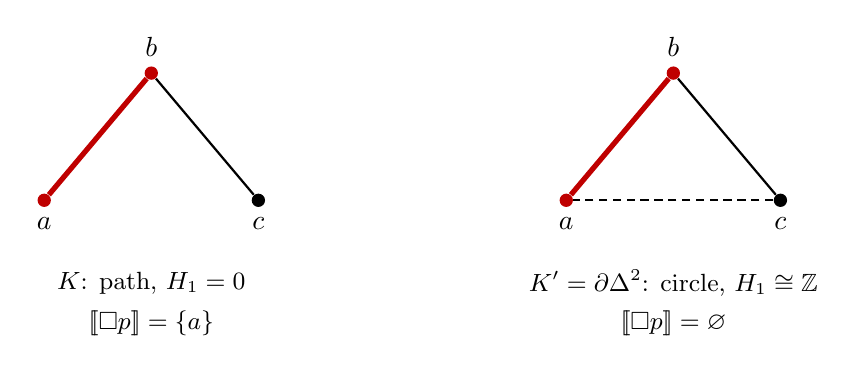
\begin{tikzpicture}[scale=1.7,
    vtx/.style={circle,fill=black,inner sep=1.7pt},
    onp/.style={circle,fill=red!75!black,inner sep=1.7pt},
    lbl/.style={font=\small}]
  \begin{scope}
    \node[onp,label=below:$a$] (a) at (0,0) {};
    \node[onp,label=above:$b$] (b) at (0.8,0.95) {};
    \node[vtx,label=below:$c$] (c) at (1.6,0) {};
    \draw[line width=1.9pt,red!75!black] (a) -- (b);
    \draw[thick] (b) -- (c);
    \node[lbl] at (0.8,-0.62) {$K$: path, $H_1=0$};
    \node[lbl] at (0.8,-0.92) {$\llbracket\Box p\rrbracket=\{a\}$};
  \end{scope}
  \begin{scope}[xshift=3.9cm]
    \node[onp,label=below:$a$] (a2) at (0,0) {};
    \node[onp,label=above:$b$] (b2) at (0.8,0.95) {};
    \node[vtx,label=below:$c$] (c2) at (1.6,0) {};
    \draw[line width=1.9pt,red!75!black] (a2) -- (b2);
    \draw[thick] (b2) -- (c2);
    \draw[thick,densely dashed] (c2) -- (a2);
    \node[lbl] at (0.8,-0.62) {$K'=\partial\Delta^2$: circle, $H_1\cong\mathbb{Z}$};
    \node[lbl] at (0.8,-0.92) {$\llbracket\Box p\rrbracket=\varnothing$};
  \end{scope}
\end{tikzpicture}
\caption{The atom \(\llbracket p\rrbracket=\{a,b,ab\}\) (highlighted) in two
complexes.  The dashed edge \(ac\) closes the cycle.  The generated
\(\Box\)-free reducts are isomorphic Heyting algebras, but \(ac\) is a coface of
\(a\) lying outside \(\llbracket p\rrbracket\), which empties
\(\llbracket\Box p\rrbracket\) on the circle.}
\label{fig:path-vs-circle}
\end{figure}

\begin{rem}[The reduct forgets structure]
\label{rem:reduct-forgets}
Example~\ref{ex:path-vs-circle} is the local witness of the phenomenon that
Theorem~\ref{thm:no-go} makes precise.  Propositional evaluation collapses a
complex into the Heyting subalgebra its valuations generate, and distinct
geometric structures can generate \emph{isomorphic} subalgebras; the reduct is
therefore not faithful to the face incidence data.  The coface quantifier in
Definition~\ref{def:forcing}(7) reads that discarded data back off the complex.
We stress that the isomorphism is claimed only for the subalgebra
\emph{generated by the atomic valuations}, not for the full lattice of
subcomplexes: the latter recovers the face poset of \(K\) and would already
separate \(K\) from \(K'\).
\end{rem}

This result subsumes Theorem~\ref{thm:geometry-inert}: the local inertness established there is recovered here as the special case of the joint classification, and the additional content of the present theorem lies in the classification it yields.

\begin{thm}[No-Go]
\label{thm:no-go}
For every realising class \(\mathcal{C}\), the set of \(\mathcal{L}_0\)-formulas
valid on all filtrations in \(\mathcal{C}\) is exactly IPC:
\(\mathrm{Log}(\mathcal{C})=\mathrm{IPC}\).
\end{thm}

\proof
\emph{Soundness.}  Every member of \(\mathcal{C}\) is a filtration in the sense
of Definition~\ref{def:filtration}, so \(\mathrm{IPC}\subseteq
\mathrm{Log}(\mathcal{C})\) by Theorem~\ref{thm:soundness}.

\emph{Completeness.}  Let \(\varphi\) be an \(\mathcal{L}_0\)-formula with
\(\nvdash_{\mathrm{IPC}}\varphi\).  By the Kripke completeness of IPC with
respect to finite rooted posets \cite{chagrovzakharyaschev1997} there are a
finite rooted poset \((W,\le)\) with root \(w_0\), a monotone valuation
\(\Vdash^{K}\), and \(w_0\nVdash^{K}\varphi\).  Since \(\mathcal{C}\) is
realising, choose \((K_t)_{t\in W}\in\mathcal{C}\) whose stage map is an
order-embedding of \(W\).  Define a valuation on this filtration by
\[
  \mathrm{val}(p,t)\;:=\;
  \begin{cases}
    K_t, & t\Vdash^{K}p,\\[2pt]
    \emptyset, & \text{otherwise.}
  \end{cases}
\]
This is persistent (Definition~\ref{def:persistent-valuation}): if \(s\le t\)
and \(s\Vdash^{K}p\) then \(t\Vdash^{K}p\) by monotonicity of \(\Vdash^{K}\),
and \(K_s\subseteq K_t\) by monotonicity of the filtration.  The valuation is
two-valued, so Theorem~\ref{thm:two-valued-stability} gives, for every stage
\(t\), every \(\sigma\in K_t\) and every \(\mathcal{L}_0\)-formula \(\psi\),
\[
  t\Vdash_\sigma\psi \iff t\Vdash^{K}\psi .
\]
Taking \(\psi=\varphi\), \(t=w_0\) and any \(\sigma\in K_{w_0}\) (nonempty by
Definition~\ref{def:realising-class}) yields \(w_0\nVdash_\sigma\varphi\).
Hence \(\varphi\notin\mathrm{Log}(\mathcal{C})\).
\qed

\paragraph{Scope of the no-go theorem.}
Theorem~\ref{thm:no-go} concerns the modality-free language
$\mathcal{L}_0$ and classes satisfying Definition~\ref{def:realising-class},
under the hypotheses stated in the theorem. Its conclusion must not be
extended to arbitrary classes of geometric models. In particular, a geometric
restriction can be covered by this theorem only when the resulting class still
satisfies those hypotheses.

\begin{rem}[The result is fragment-specific]
Over \(\mathcal{L}_\Box\) the no-go theorem fails: \(\Box\varphi\to\varphi\) is
valid on every realising class, since \(\Box A\subseteq A\) by
Proposition~\ref{prop:modal-profile}(4), yet it is not a theorem of IPC.
Theorem~\ref{thm:no-go} applies precisely to the \(\mathcal{L}_0\)-fragment.
\end{rem}

\begin{lem}[Padding Lemma]
\label{lem:padding}
Let \(P\) be an operation on finite simplicial complexes such that
\begin{enumerate}
  \item \(K\subseteq P(K)\) (\emph{expansive});
  \item \(K\subseteq K' \Rightarrow P(K)\subseteq P(K')\) (\emph{monotone});
  \item \(K\subsetneq K' \Rightarrow P(K)\subsetneq P(K')\) (\emph{strict}).
\end{enumerate}
If a class \(\mathcal{C}\) contains the stagewise image \((P(K_t))_{t\in T}\) of
every finite monotone filtration \((K_t)_{t\in T}\) with nonempty stages, then
\(\mathcal{C}\) is realising, and hence
\(\mathrm{Log}(\mathcal{C})=\mathrm{IPC}\).
\end{lem}

\proof
Let \((W,\le)\) be a finite poset.  By Lemma~\ref{lem:filtration-realization}
there is a finite monotone filtration \((K_t)_{t\in W}\) with nonempty stages
whose stage map is an order-embedding.  By (ii) the family
\((P(K_t))_{t\in W}\) is again monotone, by (i) its stages are nonempty, and by
(iii) the stage map remains an order-embedding.  By hypothesis
\((P(K_t))_{t\in W}\in\mathcal{C}\), so \(\mathcal{C}\) is realising; the
identification of the logic is Theorem~\ref{thm:no-go}.
\qed

\begin{cor}[Geometric properties are inert]
\label{cor:geometry-list}
Over \(\mathcal{L}_0\), each of the following classes yields exactly IPC.
\begin{enumerate}
  \item \emph{Connectedness and contractibility.}  Take
  \(P(K)=K\ast\{v\}\), the cone on a fresh vertex \(v\); \(P\) is expansive,
  monotone and strict, and every \(P(K)\) is contractible, hence connected.
  \item \emph{Lower dimension bounds \(\dim\ge m\).}  Take
  \(P(K)=K\ast\Delta^{m}\) on a fresh vertex set; then
  \(\dim P(K)\ge m\), and \(P\) again satisfies
  Lemma~\ref{lem:padding}(i)--(iii).
  \item \emph{Any conjunction of the above}, by composing the two joins.
\end{enumerate}
Note that padding raises dimension, so it cannot be used to realise an
\emph{upper} dimension bound; classes defined by \(\dim\le m\) are treated by
the vertex-growth analysis of Theorem~\ref{thm:bdn}.  This answers the question
posed in the Introduction: geometry alone cannot move the
\(\mathcal{L}_0\)-logic beyond IPC.
\end{cor}

\subsection{Bounding vertex growth: the logics \texorpdfstring{$\mathbf{BD}_n$}{BDn}}

\begin{defi}[Depth and the axioms \texorpdfstring{$\mathrm{bd}_n$}{bdn}]
\label{def:bdn}
A poset \((T,\le)\) has \emph{depth} \(\le n\) if it contains no chain
\(t_1<t_2<\dots<t_{n+1}\).  Define
\[
  \mathrm{bd}_1 \;:=\; p_1\vee\neg p_1,
  \qquad
  \mathrm{bd}_{k+1} \;:=\; p_{k+1}\vee\bigl(p_{k+1}\to \mathrm{bd}_k\bigr),
\]
and let \(\mathbf{BD}_n := \mathrm{IPC}+\mathrm{bd}_n\).  Then
\(\mathbf{BD}_n\) is sound and complete with respect to the Kripke frames of
depth \(\le n\), has the finite model property, and is decidable
\cite{chagrovzakharyaschev1997}.
\end{defi}

\begin{thm}
\label{thm:bdn}
Fix \(n\ge 1\) and let \(\mathcal{C}_n\) be the class of finite monotone
filtrations \((K_t)_{t\in T}\) such that
\begin{enumerate}
  \item every stage is nonempty;
  \item \(|V(K_s)|<|V(K_t)|\) whenever \(s<t\) (strict vertex growth);
  \item \(|V(K_t)|\le n\) for all \(t\in T\).
\end{enumerate}
Then
\[
  \mathrm{Log}(\mathcal{C}_n)\;=\;\mathbf{BD}_n .
\]
\end{thm}

\proof
\emph{Soundness.}  Let \((K_t)_{t\in T}\in\mathcal{C}_n\).  If
\(t_1<\dots<t_{k}\) is a chain in \(T\), then (ii) makes
\(|V(K_{t_1})|<\dots<|V(K_{t_k})|\) a strictly increasing sequence of integers
lying in \(\{1,\dots,n\}\) by (i) and (iii); hence \(k\le n\) and \((T,\le)\)
has depth \(\le n\).  Fix \(\sigma\) and put
\(T_\sigma=\{t\in T:\sigma\in K_t\}\), an up-set of \(T\), so
\(\mathrm{depth}(T_\sigma)\le n\) as well.  The forcing clauses evaluate
\(t\Vdash_\sigma\cdot\) by quantifying over \(\{t'\in T_\sigma: t'\ge t\}\), so
\((T_\sigma,\le)\) together with \(t\mapsto[\sigma\in\mathrm{val}(p,t)]\) is an
ordinary Kripke model of depth \(\le n\); by
Definition~\ref{def:bdn}, \(\mathrm{bd}_n\) is forced there.  Since
\(\sigma\) and \(t\) were arbitrary, \(\mathbf{BD}_n\subseteq
\mathrm{Log}(\mathcal{C}_n)\).

\emph{Completeness.}  Let \(\nvdash_{\mathbf{BD}_n}\varphi\).  By the finite
model property of \(\mathbf{BD}_n\) there are a finite rooted poset
\((W,\le)\) of depth \(\le n\) with root \(w_0\), a monotone valuation
\(\Vdash^{K}\), and \(w_0\nVdash^{K}\varphi\).  For \(t\in W\) let
\[
  d(t)\;:=\;\max\{\,k \;:\; \exists\, t_1<\dots<t_k=t \text{ in } W\,\},
\]
so \(1\le d(t)\le n\), and \(s<t \Rightarrow d(s)<d(t)\) because any chain
ending at \(s\) extends by \(t\).  Fix vertices \(v_1,\dots,v_n\) and set
\[
  K_t \;:=\; \mathcal{P}_{\neq\emptyset}\bigl(\{v_1,\dots,v_{d(t)}\}\bigr),
\]
the full simplex on the first \(d(t)\) vertices together with all its faces.
Then \(K_t\neq\emptyset\); \(s\le t\Rightarrow K_s\subseteq K_t\), so the
filtration is monotone; \(s<t\Rightarrow |V(K_s)|=d(s)<d(t)=|V(K_t)|\), giving
strict growth; and \(|V(K_t)|\le n\).  Hence
\((K_t)_{t\in W}\in\mathcal{C}_n\).  Equip it with the two-valued valuation
\(\mathrm{val}(p,t)=K_t\) if \(t\Vdash^{K}p\) and \(\emptyset\) otherwise,
which is persistent as in the proof of Theorem~\ref{thm:no-go}.  By
Theorem~\ref{thm:two-valued-stability}, \(t\Vdash_\sigma\psi\iff
t\Vdash^{K}\psi\) for all \(t\), all \(\sigma\in K_t\) and all \(\psi\); with
\(\psi=\varphi\) and \(t=w_0\) this refutes \(\varphi\) in a model from
\(\mathcal{C}_n\).  Therefore
\(\mathrm{Log}(\mathcal{C}_n)\subseteq\mathbf{BD}_n\).
\qed

\paragraph{Relation to the no-go theorem.}
The comparison with Theorem~\ref{thm:no-go} depends on the hypotheses
imposed on the respective model classes. In particular, the no-go conclusion
cannot be transferred to the restricted class considered here without checking
the realisation requirement and the remaining hypotheses of that theorem.

\begin{figure}[htbp]
\centering
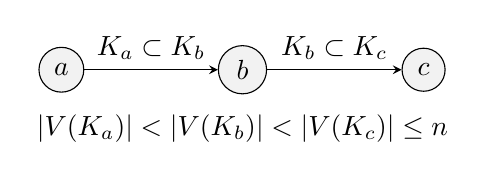
\begin{tikzpicture}[scale=1.15,>=stealth]
  \node[circle,draw,fill=gray!10] (a) at (0,0) {$a$};
  \node[circle,draw,fill=gray!10] (b) at (2,0) {$b$};
  \node[circle,draw,fill=gray!10] (c) at (4,0) {$c$};
  \draw[->] (a) -- node[above] {$K_a\subset K_b$} (b);
  \draw[->] (b) -- node[above] {$K_b\subset K_c$} (c);
  \node at (2,-0.65) {$|V(K_a)|<|V(K_b)|<|V(K_c)|\le n$};
\end{tikzpicture}
\caption{A representative bounded-depth filtration: strict vertex growth forces every chain of stages to have length at most $n$.}
\label{fig:bounded-depth-filtration}
\end{figure}

\begin{rem}[Decidability]
Since \(\mathbf{BD}_n\) has the finite model property and is decidable
\cite{chagrovzakharyaschev1997}, Theorem~\ref{thm:bdn} transfers decidability
to the geometric side: validity of an \(\mathcal{L}_0\)-formula on
\(\mathcal{C}_n\) is decidable.
\end{rem}

\begin{rem}[A single classification]
\label{rem:joint-classification}
Theorems~\ref{thm:no-go} and~\ref{thm:bdn} are two halves of one statement.
Without a constraint on vertex growth the logic is exactly IPC, whatever
geometric conditions are imposed on the stages; bounding the vertex sets by
\(n\) under strict growth pins down exactly \(\mathbf{BD}_n\).  What moves the
logic is combinatorial capacity, not shape.
\end{rem}

\begin{rem}[No-Go vs.\ \texorpdfstring{$\mathbf{BD}_n$}{BDn}: the dividing line]
\label{rem:no-go-vs-bdn}
Theorem~\ref{thm:no-go} applies to \emph{realising} classes, i.e.\ those
embedding \emph{every} finite poset.  The class \(\mathcal{C}_n\) is not
realising: a chain \(t_1<\dots<t_{n+1}\) would require \(n+1\) strictly
increasing nonempty vertex sets of size \(\le n\), which is impossible.  So
\(\mathcal{C}_n\) escapes Theorem~\ref{thm:no-go} exactly by lacking the
capacity to realise all posets, and the price of that escape is measured by
\(\mathrm{bd}_n\).
\end{rem}


\section{Stage-Local Invariants and Their Limits}
\label{sec:neg}

\subsection{The gap between the two negations}
\label{subsec:negation-gap}

\begin{prop}
\label{prop:negation-gap}
For any subcomplex \(p\in\mathrm{Sub}(K)\):
\begin{enumerate}
  \item \(\neg_H p \subseteq \neg_{\mathrm{alg}} p\);
  \item equality holds iff \(\neg_{\mathrm{alg}} p = K\setminus p\) is closed
  under faces, i.e.\ iff \(\neg_{\mathrm{alg}} p\in\mathrm{Sub}(K)\);
  \item in general \(\neg_H p\) is the largest subcomplex contained in the
  set-theoretic complement.
\end{enumerate}
\end{prop}

\proof
By Corollary~\ref{cor:heyting-negation},
\(\neg_H p=\bigcup\{r\in\mathrm{Sub}(K)\mid r\cap p=\emptyset\}\).  Any such
\(r\) satisfies \(r\subseteq K\setminus p=\neg_{\mathrm{alg}}p\), which gives
(i) and (iii).  For (ii): if \(K\setminus p\) is face-closed it is itself the
largest such \(r\), so equality holds; conversely equality forces
\(K\setminus p=\neg_H p\in\mathrm{Sub}(K)\).
\qed

\begin{exa}
\label{ex:negation-gap}
Let \(K\) be the filled triangle on \(\{a,b,c\}\),
\[
K=\bigl\{\{a\},\{b\},\{c\},\{a,b\},\{a,c\},\{b,c\},\{a,b,c\}\bigr\},
\]
and \(p=\{\{a\},\{b\},\{a,b\}\}\).  Then
\(\neg_{\mathrm{alg}}p=K\setminus p=\{\{c\},\{a,c\},\{b,c\},\{a,b,c\}\}\),
which is not a subcomplex: \(\{a,c\}\) is present while its face \(\{a\}\) is
not.  Heyting negation keeps only the face-closed part,
\[
\neg_H p=\bigl\{\{c\}\bigr\},
\]
since any subcomplex disjoint from \(p\) can contain none of
\(\{a,c\},\{b,c\},\{a,b,c\}\).  Hence
\(\neg_H p\subsetneq\neg_{\mathrm{alg}}p\), the offending simplices being
exactly those three.
\end{exa}

\subsection{Graded negation along a filtration}
\label{subsec:graded-negation}

\begin{defi}[Graded negation]
\label{def:graded-negation}
For a filtration \((K_t)_{t\in T}\) with persistent valuation, and
\(p_t:=\mathrm{val}(p,t)\), define the \emph{graded negation}
\[
  \neg^{(t)}p \;:=\; \neg_H^{K_t}p_t,
\]
the Heyting negation computed inside the single stage \(K_t\).
\end{defi}

\begin{prop}
\label{prop:graded-antitone}
If \(s\le t\) then \(\neg^{(t)}p\cap K_s\subseteq\neg^{(s)}p\).
\end{prop}

\proof
Put \(r:=\neg^{(t)}p\cap K_s\).  Both factors are subcomplexes and
\(\mathrm{Sub}(K_s)\) is closed under intersection with subcomplexes of
\(K_t\), so \(r\in\mathrm{Sub}(K_s)\).  By persistence
(Definition~\ref{def:persistent-valuation}) \(p_s\subseteq p_t\), and
\(\neg^{(t)}p\cap p_t=\emptyset\) by Corollary~\ref{cor:heyting-negation};
hence \(r\cap p_s\subseteq \neg^{(t)}p\cap p_t=\emptyset\).  Thus \(r\) is a
subcomplex of \(K_s\) disjoint from \(p_s\), and maximality of
\(\neg_H^{K_s}p_s\) gives \(r\subseteq\neg^{(s)}p\).
\qed

\begin{rem}[Reading of the grading]
\label{rem:graded-negation-status}
The index in \(\neg^{(t)}\) is a filtration stage, not a dimension, and the
operator is antitone in it: \emph{truth grows, refutation shrinks}.  Being
stage-local, \(\neg^{(t)}\) need not agree with the interpretation of \(\neg\)
in the filtration model, which quantifies over all later stages; the
discrepancy is exactly the gap isolated in
Proposition~\ref{prop:negation-gap}, and
Subsection~\ref{subsec:non-internalizable} shows that the mismatch cannot be
repaired.  The grading is therefore a diagnostic on the algebras
\(\mathrm{Sub}(K_t)\), locating the stage at which a refutation is lost; no
claim is made that it enlarges the set of validities.  The asymmetry is close
in spirit to Dummett's account of intuitionistic negation as a claim about all
available constructions \cite{dummett1977}, and the picture of a background
shifting while inference proceeds invites comparison with Wittgenstein's
river-bed \cite[\S\S96--99]{wittgenstein1969}; neither comparison is
presupposed below.
\end{rem}

\subsection{The clarity operator}
\label{subsec:clarity}

\begin{defi}[Clarity]
\label{def:clarity}
The \emph{clarity operator} on \(\mathrm{Sub}(K)\) is
\[
  \mathop{\mathrm{Cl}}(p)\;:=\;\neg_H\neg_H p .
\]
Standard Heyting-algebra facts give \(p\subseteq\mathop{\mathrm{Cl}}(p)\),
monotonicity, idempotence, and
\(\mathop{\mathrm{Cl}}(p\cap q)=\mathop{\mathrm{Cl}}(p)\cap
\mathop{\mathrm{Cl}}(q)\); hence \(\mathop{\mathrm{Cl}}\) is not merely a
closure operator but a \emph{nucleus}.  Its fixed points are the \emph{clear}
(regular) subcomplexes.
\end{defi}

\begin{prop}
\label{prop:clarity-boolean}
The clear subcomplexes form a Boolean algebra, the Booleanisation of
\(\mathrm{Sub}(K)\), with \(\wedge=\cap\), join
\(p\sqcup q:=\mathop{\mathrm{Cl}}(p\cup q)\), and negation \(\neg_H\).
\end{prop}

\proof
This is the regular-element theorem for Heyting algebras.  The SC reading:
clarity erases ambiguity at the boundary, since \(p\) is clear iff every
simplex that cannot be refuted, i.e.\ lies outside \(\neg_H p\), is already
present, so nothing hovers between \(p\) and its Heyting complement.
\qed

\begin{exa}
\label{ex:clarity}
Continue with \(K\) and \(p=\{\{a\},\{b\},\{a,b\}\}\) from
Example~\ref{ex:negation-gap}, where \(\neg_H p=\{\{c\}\}\).  Then
\[
\mathop{\mathrm{Cl}}(p)=\neg_H\{\{c\}\}
=\bigcup\bigl\{r\in\mathrm{Sub}(K)\;\big|\;r\cap\{\{c\}\}=\emptyset\bigr\}
=\bigl\{\{a\},\{b\},\{a,b\}\bigr\}=p,
\]
so \(p\) is already clear.  A genuine clarification appears for
\(r=\{\{a\},\{b\}\}\): again \(\neg_H r=\{\{c\}\}\), whence
\[
\mathop{\mathrm{Cl}}(r)=\bigl\{\{a\},\{b\},\{a,b\}\bigr\}\supsetneq r,
\]
and the edge \(\{a,b\}\) is clarified in: no subcomplex disjoint from \(r\)
excludes it, so regularisation forces it back.
\end{exa}

\begin{rem}
The clarified-in simplices of Example~\ref{ex:clarity} occupy a stable third
position: neither verified nor refutable, yet not revisable in the manner of
the mixed region.  Within the algebra they play a role structurally analogous
to the hinge propositions of \cite{wittgenstein1969}, with the difference that
membership is decidable from the face poset.  We stress that
\(\mathop{\mathrm{Cl}}\) carries no temporal reading: by
Definition~\ref{def:clarity} it is a nucleus computed inside a single stage.
\end{rem}

\begin{rem}[Clarity adds no deductive strength]
\label{rem:clarity-no-strength}
\(\mathop{\mathrm{Cl}}\) is definable in \(\mathcal{L}_0\), being
\(\neg\neg\); adding it as a primitive validates no new formulas.  Its
interest is structural: it exposes the regular subcomplexes and the geometric
content of double-negation stability (Proposition~\ref{prop:clarity-boolean}).
\end{rem}

\subsection{Non-internalisability of stage-local negation}
\label{subsec:non-internalizable}

\begin{prop}
\label{prop:non-internalizable}
There is no \(\mathcal{L}_0\)-formula \(\psi(p)\) such that
\(\llbracket\psi(p)\rrbracket_t=\neg^{(t)}p\) in every filtration model at every
stage \(t\).  More generally, no operator that is strictly antitone in the
stage index on some model can be the semantics of a connective.
\end{prop}

\proof
Heredity (Lemma~\ref{lem:heredity}) requires truth sets to be \emph{monotone}
in the stage index: if \(s\le t\) then
\(\llbracket\psi\rrbracket_s\subseteq\llbracket\psi\rrbracket_t\).  Graded
negation violates this.  Take \(T=\{0<1\}\), \(K_0=K_1=\{\{a\}\}\), and
\(\mathrm{val}(p,0)=\emptyset\), \(\mathrm{val}(p,1)=\{\{a\}\}\); this
valuation is persistent.  Then
\[
  \neg^{(0)}p=\neg_H^{K_0}\emptyset=K_0=\{\{a\}\},
  \qquad
  \neg^{(1)}p=\neg_H^{K_1}\{\{a\}\}=\emptyset .
\]
If some \(\psi\) had \(\llbracket\psi\rrbracket_t=\neg^{(t)}p\), then
\(0\Vdash_{\{a\}}\psi\) while \(0\le 1\) and \(\{a\}\in K_1\), so heredity
would give \(1\Vdash_{\{a\}}\psi\), contradicting
\(\llbracket\psi\rrbracket_1=\emptyset\).  Hence no such \(\psi\) exists.  The
general claim follows by the same argument applied to any strictly antitone
family.
\qed

\begin{rem}
This is a second, smaller no-go result: no stage-local operator can be a
propositional connective of SC-Logic.  \(\neg^{(t)}\) is best read as a
meta-level invariant stratifying a single intuitionistic negation into a
persistence-indexed hierarchy.  It motivates a genuine modal operator
\(\Box\) (Section~\ref{sec:box}), whose heredity is built into its definition
rather than imposed pointwise.
\end{rem}



%============================================================
% Section 8 : Robust Topological Queries under Filtration
% Self-contained. Requires: amsmath, amssymb, amsthm.
% def:forcing, def:clarity, prop:fmp, cor:decidability, sec:kripke.
%============================================================
\section{Robust Topological Queries under Filtration}
\label{sec:application}

This section illustrates filtration queries using Heyting negation and the
clarity operator $\mathop{\mathrm{Cl}}=\neg_H\neg_H$ of
Definition~\ref{def:clarity}. The examples contrast the unstable set-theoretic
complement with the internal, face-closed operations of SC-Logic.


\subsection{The flickering of the classical complement}

A set-theoretic complement of a subcomplex need not be face-closed, whereas
Heyting negation remains internal to $\mathrm{Sub}(K)$.

\begin{exa}[The set-complement is not a subcomplex]
\label{ex:complement-not-subcomplex}
Let $K$ be the filled triangle on vertices $\{a,b,c\}$, i.e.
\[
K=\bigl\{\{a\},\{b\},\{c\},\{a,b\},\{b,c\},\{a,c\},\{a,b,c\}\bigr\},
\]
and let $p=\{\{a\}\}$ be the subcomplex consisting of the single vertex
$a$. The set-theoretic complement is
\[
1\setminus p=\bigl\{\{b\},\{c\},\{a,b\},\{b,c\},\{a,c\},\{a,b,c\}\bigr\},
\]
which is \emph{not} a subcomplex: it contains the edge $\{a,b\}$ but not
its face $\{a\}$. By contrast, the Heyting negation
(Corollary~\ref{cor:heyting-negation}) returns the largest subcomplex
disjoint from $p$,
\[
\neg_H p=\{\{b\},\{c\},\{b,c\}\},
\]
which is a genuine subcomplex. Thus $\neg_H p\subsetneq 1\setminus p$,
and only $\neg_H p$ is a legitimate object of the logic.
\end{exa}

For a stage $t$, let $C_t:=K_t\setminus\mathrm{val}(p,t)$ and let $D_t$
denote its defect set. The next example records the resulting flicker.

\begin{exa}[Flickering of the set-complement]
\label{ex:flickering-complement}
Let $T=\{1,2,3\}$ and let $F=(K_t)_{t\in T}$ be the filtration on the
vertex set $\{a,b\}$ given by
\[
K_1=\bigl\{\{a\},\{b\}\bigr\},
\qquad
K_2=K_3=K_1\cup\bigl\{\{a,b\}\bigr\},
\]
with the persistent valuation
\[
\mathrm{val}(p,1)=\mathrm{val}(p,2)=\bigl\{\{a\}\bigr\},
\qquad
\mathrm{val}(p,3)=\bigl\{\{a\},\{a,b\}\bigr\}.
\]
Both $t\mapsto K_t$ and $t\mapsto\mathrm{val}(p,t)$ are monotone, and
each $\mathrm{val}(p,t)$ is a subcomplex of $K_t$. The set-complements
are
\[
C_1=\bigl\{\{b\}\bigr\},
\qquad
C_2=\bigl\{\{b\},\{a,b\}\bigr\},
\qquad
C_3=\bigl\{\{b\}\bigr\},
\]
whence
\[
D_1=\varnothing,
\qquad
D_2=\bigl\{\{a,b\}\bigr\},
\qquad
D_3=\varnothing .
\]
Indeed $C_2$ contains the edge $\{a,b\}$ but not its face $\{a\}$,
while $C_1$ and $C_3$ are genuine subcomplexes. The set-complement
therefore \emph{flickers} between well-formed and ill-formed states as
the filtration proceeds, so no query built on it can be stable in $t$.
\end{exa}

By Corollary~\ref{cor:heyting-negation}, Heyting negation always remains in
$\mathrm{Sub}(K_t)$, so its defect set is empty.



\subsection{A sensor-network filtration}
\label{subsec:sensor-network}
For illustration, take six sensors on a cyclic index set and a three-stage
Vietoris--Rips filtration $F=(K_t)_{t\in T}$, $T=\{0,1,2\}$, in which a
transient one-dimensional hole appears at the middle stage.
\[
\{s_{i_0},\dots,s_{i_k}\}\in K_t
\iff
\max_{0\le a<b\le k}\, d_{\mathrm{cyc}}(i_a,i_b)\le t,
\qquad
d_{\mathrm{cyc}}(i,j)=\min\bigl(|i-j|,6-|i-j|\bigr).
\]
\begin{itemize}
  \item $K_0$: vertices only.
  \item $K_1$: the hexagonal cycle.
  \item $K_2$: the cycle filled by the prescribed triangles.
\end{itemize}
The inclusions $K_0\subseteq K_1\subseteq K_2$ are monotone, so this is a
filtration in the sense of Definition~\ref{sec:kripke}.
\[
\{s_{i_0},\dots,s_{i_k}\}\in K_t
\iff
\max_{0\le a<b\le k}\, d_{\mathrm{cyc}}(i_a,i_b)\le t,
\qquad
d_{\mathrm{cyc}}(i,j)=\min\bigl(|i-j|,\,6-|i-j|\bigr).
\]
Explicitly:
\begin{itemize}
  \item $K_0$: the six vertices only (all pairwise distances $>0$).
  \item $K_1$: the vertices together with the six ``short'' edges
        $\{s_i,s_{i+1}\}$, forming the hexagonal cycle $\partial H$
        (a $1$-dimensional complex with one $1$-cycle).
  \item $K_2$: all vertices, all edges $\{s_i,s_j\}$ with
        $d_{\mathrm{cyc}}(i,j)\le 2$, and \emph{all} triangles
        $\{s_i,s_j,s_k\}$ whose three indices are pairwise within cyclic
        distance $2$. Concretely the triangles are exactly the six
        ``fans'' $\{s_{i-1},s_i,s_{i+1}\}$ together with the two
        ``alternating'' triangles $\{s_0,s_2,s_4\}$ and
        $\{s_1,s_3,s_5\}$.
\end{itemize}
The inclusions $K_0\subseteq K_1\subseteq K_2$ are monotone, so $F$ is a
filtration in the sense of Definition~\ref{sec:kripke}, and $(T,\le)$ is
its filtration frame.

\begin{rem}
The one-dimensional hole of $K_1$ (the hexagonal loop $\partial H$) is
the topological feature we wish to query. It is \emph{transient}: it is
born at $t=1$ and dies at $t=2$ once enough triangles fill the disk. A
robust query language must report this feature only where it genuinely
persists, without spurious appearances caused by non-subcomplex
artefacts.
\end{rem}

\subsection{Robustness: stability and regularity}

Recall from Lemma~\ref{lem:truth-set-subcomplex} that, for a persistent
valuation satisfying face-heredity of atoms, every truth set
$\llbracket\varphi\rrbracket_t$ is a subcomplex of $K_t$. This is the
structural guarantee that Example~\ref{ex:complement-not-subcomplex}
shows a set-theoretic complement cannot provide.

We now formalise two guarantees. The first says that queries built from
Heyting negation are \emph{monotone-stable}: once a negated feature is
established at a stage, growth of the complex can only shrink its
refutation set in a controlled way, never fabricate new cells outside
$Sub(K)$. The second says that \emph{clear} queries are exactly the
regular (double-negation-stable) subcomplexes, and that clarity is a
genuine idempotent that already fixes every Heyting-negated region.

\begin{prop}[Monotone stability of the persistent fragment]
\label{prop:persistent-stability}
Let $p\in Sub(K)$ and let $s\le t$ in $T$. Then
\[
\neg_H^{K_t}p\ \cap\ K_s\ \subseteq\ \neg_H^{K_s}p .
\]
Equivalently, the graded negation $\neg^{(t)}p$ is antitone in $t$: a
cell refuted at stage $t$ that already exists at stage $s$ was refuted
at stage $s$ as well. In particular no cell can be refuted, un-refuted,
and refuted again along the filtration; the negated fragment does not
flicker.
\end{prop}

\proof
By Corollary~\ref{cor:heyting-negation}, $\neg_H^{K_t}p$ is the largest
subcomplex of $K_t$ disjoint from $p$. Let
$\sigma\in\neg_H^{K_t}p\cap K_s$. Then $\sigma\in K_s$ and $\sigma$ lies
in a subcomplex of $K_t$ disjoint from $p$; restricting that subcomplex
along the inclusion $K_s\subseteq K_t$ yields a subcomplex of $K_s$
containing $\sigma$ and still disjoint from $p$. By maximality of
$\neg_H^{K_s}p$ we obtain $\sigma\in\neg_H^{K_s}p$. This is exactly the
antitonicity of graded negation, and it forbids the flicker pattern
``refuted at $s$, not at some $u$ with $s\le u\le t$, refuted again at
$t$'': the middle failure at $u$ would contradict the inclusion applied
to the pair $u\le t$.
\qed

\begin{prop}[Regularity of clear queries]
\label{prop:clarity-regular}
For every $p\in Sub(K)$:
\begin{enumerate}
  \item $C(p)=\neg_H\neg_H p$ is the smallest regular (clear) subcomplex
        containing $p$, and $C(C(p))=C(p)$.
  \item \textbf{(Triple-negation law.)} Every Heyting-negated region is
        already clear:
        \[
        \neg_H\neg_H\neg_H p=\neg_H p,
        \qquad\text{equivalently}\qquad
        C(\neg_H p)=\neg_H p .
        \]
  \item $C(p)$ is disjoint from $\neg_H p$, and $C(p)=\neg_{\mathrm{alg}}
        \neg_{\mathrm{alg}}p$ holds iff the algebraic double complement
        is face-closed, i.e.\ already a subcomplex.
\end{enumerate}
\end{prop}

\proof
\emph{(1)} By Definition~\ref{def:clarity}, $C=\neg_H\neg_H$ is a nucleus
on the Heyting algebra $\mathrm{Sub}(K)$: it is inflationary ($p\subseteq C(p)$),
monotone, and idempotent. Its fixpoints are the regular elements, and
$C(p)$ is the least such element above $p$.

\emph{(2)} In any Heyting algebra one has $p\le\neg_H\neg_H p$; applying
the antitone map $\neg_H$ reverses the inequality to
$\neg_H\neg_H\neg_H p\le\neg_H p$. Conversely, instantiating
$p\le\neg_H\neg_H p$ at $\neg_H p$ gives
$\neg_H p\le\neg_H\neg_H(\neg_H p)=\neg_H\neg_H\neg_H p$. The two
inequalities force equality $\neg_H\neg_H\neg_H p=\neg_H p$. Reading the
left-hand side as $C(\neg_H p)$ yields $C(\neg_H p)=\neg_H p$; thus
$\neg_H p$ is a fixpoint of $C$, i.e.\ a clear subcomplex, and applying
$C$ to it changes nothing.

\emph{(3)} Since $\neg_H p$ is the largest subcomplex disjoint from $p$
and $C(p)=\neg_H(\neg_H p)$ is disjoint from $\neg_H p$ by the defining
adjunction $r\cap(\neg_H p)=\varnothing\iff r\subseteq\neg_H\neg_H p$,
disjointness \(\mathop{\mathrm{Cl}}(p)\cap\neg_H p=\varnothing\) is immediate. Finally, by
Proposition~\ref{prop:coface-removal} the algebraic and Heyting negations coincide exactly.
when the algebraic complement is face-closed, giving the stated
equality condition.
\qed

\subsection{Querying the transient hole}

We can now phrase the intended topological query correctly. The
naive attempt is to ask for ``the covered region and its complementary
hole'' via $C(\neg c)$, where $c\in Sub(K)$ is the covered subcomplex.
By the triple-negation law
(Proposition~\ref{prop:clarity-regular}(2)) this is a trap:
\[
C(\neg_H c)=\neg_H\neg_H\neg_H c=\neg_H c,
\]
so the clarity pass does nothing and the ``interesting'' object collapses
to the plain negation. The genuinely interesting object is the
\emph{stable core of the covered region} itself:
\[
\varphi_{\mathrm{core}}:=\mathop{\mathrm{Cl}}(c)=\neg_H\neg_H c .
\]
The covered region $c$ has this stable core $\mathop{\mathrm{Cl}}(c)$, obtained by
stripping boundary-adherent cells that fail to be double-negation
stable. Its Heyting complement $\neg_H c$ is the uncovered region;
by the triple-negation law $\neg_H\neg_H\neg_H c=\neg_H c$, this region
is \emph{itself} regular and requires no further clarity pass.

Concretely, in the filtration of Section~\ref{subsec:sensor-network} let \(c=K_1\) record ``a short
communication link exists.'' Then $\neg_H c$ selects the largest
subcomplex carrying \emph{no} short link, and \(\mathop{\mathrm{Cl}}(c)=\neg_H\neg_H c\)
returns the double-negation-stable core of the linked region. By
Proposition~\ref{prop:persistent-stability} the negated fragment
$\neg^{(t)}c$ is antitone: as the disk fills at $t=2$, the uncovered
region can only shrink, and it never reappears. The transient hole of
$K_1$ is thus reported precisely on the stages where it is
topologically real, with no flickering artefacts.
Unlike standard persistence, where stability is a \emph{post hoc} analysis of
feature longevity, SC-Logic embeds stability directly into the semantics of the
query language, rendering the persistence of the stable core
\(\mathop{\mathrm{Cl}}(c)\) a primitive logical property.

\subsection{Failure of a classical set-complement semantics}
\label{subsec:why-not-classical}

Three properties jointly account for the robustness of SC-Logic, none of
which is available to a classical set-complement semantics.
\begin{enumerate}
  \item \textbf{Closure inside $Sub(K)$.} By
        Corollary~\ref{cor:heyting-negation} and
        Example~\ref{ex:complement-not-subcomplex}, $\neg_H$ always
        returns a subcomplex, whereas $1\setminus p$ generally does not.
        Every intermediate query is therefore a legitimate topological
        object.
  \item \textbf{Monotone stability.} By
        Proposition~\ref{prop:persistent-stability}, refutations are
        antitone along the filtration, so no feature flickers.
  \item \textbf{Idempotent clarity.} By
        Proposition~\ref{prop:clarity-regular}, $C=\neg_H\neg_H$ is an
        idempotent nucleus whose fixpoints are exactly the regular
        subcomplexes, and every negated region is already a fixpoint.
        Clarity acts as a \emph{logical persistence filter}.
\end{enumerate}

Because SC-Logic is decidable and enjoys the finite model property
(Proposition~\ref{prop:fmp} and Corollary~\ref{cor:decidability}), each
of these queries is effectively computable on the finite complexes
$K_t$. SC-Logic thus provides exactly the guarantees a robust
topological query language requires: validity, stability, and
computability, in a single Heyting-algebraic package.

\section{Comparison with Related Frameworks}
\label{sec:comparison}

The semantics developed above sits at the intersection of three traditions:
topological semantics for intuitionistic logic, qualitative spatial reasoning,
and the use of simplicial complexes in logic and in topological data analysis.
We record precisely how the present framework relates to each, and in
particular how Theorem~\ref{thm:geometry-inert} should be read against them.

\paragraph{Topological semantics for IPC.}
Interpreting intuitionistic connectives by open sets of a topological space
goes back to Tarski~\cite{tarski1938} and to McKinsey and
Tarski~\cite{mckinseytarski1944}, who proved completeness of IPC with respect
to the open-set algebra of any separable metric space that is dense-in-itself,
in particular of \( \mathbb{R}^{n} \). Our Heyting algebra \( \mathrm{Sub}(K) \) is
\emph{combinatorial} rather than point-set: its elements are subcomplexes, a
family closed under arbitrary unions and intersections but not equal to the
opens of a topology on the underlying vertex set, and the induced negation
\( \neg_{H} \) is computed by coface removal rather than by taking the
interior of a set-complement (Proposition~\ref{prop:coface-removal},
Corollary~\ref{cor:heyting-negation}). The practical gain is effectivity:
implication, negation and clarity are finite face-poset computations, whereas
the classical topological models are infinite. The price, made precise by
Theorem~\ref{thm:geometry-inert}, is that this extra
structure buys no extra validities.

\paragraph{Kripke frames and Esakia duality.}
Kripke~\cite{kripke1965} gave the relational semantics for IPC in which
formulas denote upward-closed sets of a poset, and Esakia
duality~\cite{esakia2019} identifies Heyting algebras with certain ordered
topological spaces. Filtration frames (Definition~\ref{def:filtration-frame})
are Kripke frames of a restricted shape, stages organised by a monotone
filtration parameter, and persistent valuations
(Definition~\ref{def:persistent-valuation}) are exactly the valuations for
which truth is hereditary along the filtration
(Lemma~\ref{lem:heredity}). Two points are worth isolating. Restricting to
this shape does not restrict the logic: the point-filtration construction of
Definition~\ref{def:point-filtration} converts an arbitrary countermodel into
a filtration countermodel, which is what makes strong completeness
(Theorem~\ref{thm:completeness}) go through. Conversely, the face-poset
representation (Theorem~\ref{thm:subk-representation}) is a
\emph{realisability} statement in the opposite direction: not every finite
Heyting algebra arises as some \( \mathrm{Sub}(K) \), so the class of
subcomplex algebras is properly smaller than the class of finite Heyting
algebras even though it generates the same logic
(Corollary~\ref{cor:realizable-heyting}).

\paragraph{Qualitative spatial reasoning.}
Region-based spatial calculi such as RCC~\cite{randell1992} and the
modal spatial logics surveyed by Aiello, van Benthem and
Bezhanishvili~\cite{aiello2003} also reason about regions rather than points,
and also treat complementation with care. The difference is one of aim. Those
systems fix a space and axiomatise a repertoire of qualitative relations
(connection, tangency, parthood) whose logic is typically modal or
first-order. Here the space is not fixed: the object of study is a filtration,
the intended queries are monotone in the filtration parameter, and the
qualitative content is carried by graded negation
(Definition~\ref{def:graded-negation}) and by regularity
(Proposition~\ref{prop:clarity-regular}) rather than by primitive spatial
relations. In particular the flickering phenomenon of
Section~\ref{sec:application} has no counterpart in the fixed-space setting,
since it is precisely an artefact of complementation interacting with growth.

\paragraph{Clarity, nuclei and lax logic.}
The clarity operator \(\mathop{\mathrm{Cl}}\) (Definition~\ref{def:clarity})
is defined as \(\neg_H\neg_H\) and satisfies more than the axioms of a closure
operator: it is a \emph{nucleus} on the Heyting algebra \(\mathrm{Sub}(K)\),
i.e.\ an idempotent inflationary interior operator that commutes with meets.
Nuclei on Heyting algebras correspond to quotient Heyting algebras via their
fixed-point sublattice, and provide the algebraic counterpart of open
geometric morphisms in topos theory~\cite{johnstone1982}. In the propositional
setting, nuclei interpret the Lawvere-style ``lax'' modalities studied by
Fairtlough and Mendler~\cite{fairtlough1997} in the context of resource-aware
reasoning, where the modality stratifies formulas into levels of commitment or
refinement. Our use of clarity is formally analogous: clear subcomplexes are
the stable geometric cores under iterated complementation, and the nucleus
structure ensures that the sublattice of clear elements inherits the Heyting
structure. This connection suggests that the graded negations of
Section~\ref{subsec:graded-negation} admit a lax-logic reading, though we do not pursue
that interpretation here.

\paragraph{Intuitionistic modal logics.}
The operator \( \Box \) introduced in Section~\ref{sec:box} is a normal,
reflexive, non-transitive modality, i.e.\ an intuitionistic
\( \mathsf{T} \)-modality in the sense of the systems surveyed below.
Bo{\v z}i{\'c} and Do{\v s}en~\cite{bozicdosen1984} and Fischer
Servi~\cite{fischer-servi1983} introduced the standard bi-relational Kripke
semantics for normal intuitionistic modal logics; Simpson's
thesis~\cite{simpson1994} develops the proof-theoretic and semantic
foundations, Ono~\cite{ono1977} surveyed the landscape of intuitionistic
modal extensions, and Wolter and Zakharyaschev~\cite{wolterzakharyaschev1999}
give the modern algebraic and correspondence-theoretic account.  Our
\( \Box \) validates necessitation, axiom \( \mathsf{K} \) and axiom
\( \mathsf{T} \) (Proposition~\ref{prop:modal-profile}) but fails axiom
\( \mathsf{4} \) (Proposition~\ref{prop:box-not-4}), so it is strictly
weaker than the intuitionistic \( \mathsf{iS4} \) systems of
Bo{\v z}i{\'c} and Do{\v s}en~\cite{bozicdosen1984}.  We do not claim that
SC-Logic's \( \Box \) coincides with any of these systems; the comparison is
limited to the shared structural properties (normality, reflexivity,
non-transitivity), and the completeness question for \( \mathcal{L}_\Box
\) remains open (Section~\ref{sec:box}).

\paragraph{Simplicial complexes in epistemic logic.}
Simplicial complexes have recently been used as models of distributed
knowledge, where vertices are local states of processes and facets are global
configurations~\cite{goubault2021,vanditmarsch2024}. Despite the shared
combinatorial substrate, the semantics is orthogonal to ours in two respects.
Those models are \emph{modal and classical}: formulas denote sets of facets,
the connectives are Boolean, and the logical content lies in the knowledge
operators induced by the chromatic structure. Our models are
\emph{intuitionistic and non-modal}: formulas denote subcomplexes, the
connectives are the Heyting operations of \( \mathrm{Sub}(K) \), and no
epistemic reading is intended. The two frameworks are therefore best seen as
complementary uses of the same geometry, and combining them, knowledge
operators over a filtration of chromatic complexes, is a natural question
that we do not address here.

\paragraph{Filtrations and topological data analysis.}
The filtrations of Definition~\ref{def:filtration} are the standard input of
persistent homology~\cite{chazal2016}, and the presheaf-like behaviour noted in
Remark~\ref{rem:filtration-presheaf} is the same monotonicity that makes
persistence modules well behaved~\cite{bubenikscott2014}. The invariants,
however, are of different type. Persistent homology extracts
\emph{homological} invariants, barcodes of cycles, and is insensitive to the
lattice structure of subcomplexes. Our graded negations extract
\emph{order-theoretic} invariants of the same filtration: the stage from which
a query region is persistently avoided, and the stable core of a query under
the clarity nucleus (Proposition~\ref{prop:persistent-stability}). Nothing here
computes or approximates a barcode, and nothing in persistence computes
\( \neg_{H} \); the two are independent readings of one filtration, and their
interaction is left open.

\paragraph{What the inertness theorem does and does not say.}
Because the comparisons above may suggest that a richer geometry should yield a
richer logic, we state the delimitation explicitly. Theorem~\ref{thm:geometry-inert}
says that the set of formulas valid on \emph{all} filtration models is exactly
IPC, and Theorem~\ref{thm:two-valued-stability} shows that the standard
non-degeneracy conditions on complexes do not change this. It does \emph{not}
say that the geometry is irrelevant: it says that the geometry's contribution
is invisible to the propositional consequence relation and must be accessed
by one of three routes: additional \emph{language}, graded or
persistence-indexed modalities, constraints on valuations, or restriction of
the class of realising complexes to those satisfying geometric growth
conditions, the last of which yields the intermediate logics
\( \mathbf{BD}_{n} \) (Theorem~\ref{thm:bdn}, Corollary~\ref{cor:geometry-list}).
All three routes are discussed as open problems in Section~\ref{sec:conclusion}.

\section{The Spatial Modality \texorpdfstring{$\Box$}{Box}}
\label{sec:box}

\begin{rem}[Scope of the modal section]
This section is exploratory: soundness and the stated validity results are
proved, but a completeness theorem for the full modal language is not proved
here.
\end{rem}

The non-internalizability of stage-local negation (Proposition~\ref{prop:non-internalizable})
motivates a genuine modal operator \(\Box\) whose heredity is built into its
definition.  This section introduces \(\Box\) over the face poset, records its
basic properties, and states the main technical constraint imposed by padding.

\subsection{Definition and heredity}

\begin{defi}[Spatial modality \(\Box\)]
\label{def:box}
Let \((K_t)_{t\in T}\) be a monotone filtration. For \(\sigma\in K_{t'}\) write
\[
  \uparrow_{t'}\!\sigma=\{\tau\in K_{t'}\mid \tau\supseteq\sigma\},
  \qquad
  \downarrow\!\sigma=\{\tau\neq\varnothing\mid \tau\subseteq\sigma\}
\]
for the coface filter of \(\sigma\) in \(K_{t'}\) and its face closure; note
that \(\sigma\in\uparrow_{t'}\!\sigma\). For a formula \(\varphi\), define the
\emph{box-set} at stage \(t\) by
\[
  B_t(\varphi):=\{\sigma\in K_t\mid
  \forall t'\geq t:\ \uparrow_{t'}\!\sigma\subseteq
  \llbracket\varphi\rrbracket_{t'}\},
\]
and set
\[
  \llbracket\Box\varphi\rrbracket_t:=
  \mathrm{int}_{K_t}\bigl(B_t(\varphi)\bigr),
  \qquad
  \mathrm{int}_{K}(S):=\{\sigma\in K\mid \downarrow\!\sigma\subseteq S\}.
\]
Thus \(\sigma\in B_t(\varphi)\) iff \(\varphi\) holds at \(\sigma\) itself
(take \(t'=t\), \(\tau=\sigma\)) and at every coface of \(\sigma\) occurring at
any future stage. The operator \(\mathrm{int}_{K_t}\) is the interior of the
Alexandrov (down-set) topology on the face poset \(\mathcal{F}(K_t)\), so
\(\llbracket\Box\varphi\rrbracket_t\) is the largest subcomplex of \(K_t\)
contained in \(B_t(\varphi)\).
\end{defi}

\begin{lem}[Persistence of \(\Box\)]
\label{lem:box-heredity}
Let \(s \leq t\) and \(\sigma \in \llbracket \Box \varphi \rrbracket_s\).
Then \(\sigma \in \llbracket \Box \varphi \rrbracket_t\).
\end{lem}

\proof
Assume \(\sigma \in \llbracket \Box \varphi \rrbracket_s =
\mathrm{int}_{K_s}(B_s(\varphi))\).  There exists a subcomplex
\(U\subseteq K_s\) with \(\sigma\in U\subseteq B_s(\varphi)\).
Since \(s\le t\), the set of future stages shrinks:
\(\{t'\ge t\}\subseteq\{t'\ge s\}\), so
\(B_s(\varphi)\subseteq B_t(\varphi)\).  Hence
\(U\subseteq K_s\subseteq K_t\) is a subcomplex of \(K_t\) containing \(\sigma\) and
contained in \(B_t(\varphi)\), giving
\(\sigma\in\mathrm{int}_{K_t}(B_t(\varphi))=\llbracket\Box\varphi\rrbracket_t\).
\qed

\subsection{Basic properties}

\begin{prop}[Modal profile of \(\Box\)]
\label{prop:modal-profile}
Let \((K_t)_{t\in T}\) be a monotone filtration and let
\(\varphi,\psi \in \mathcal{L}_\Box\).  Then \(\Box\) is a \emph{normal}
modality validating \(\mathsf{T}\) but not \(\mathsf{4}\); semantically it is a
monotone, deflationary and \emph{non-idempotent} operator on
\(\mathrm{Sub}(K_t)\), hence not an interior operator.  Precisely:
\begin{enumerate}
  \item \emph{(Necessitation)} If \(\varphi\) is valid on the class of
        filtration models, then so is \(\Box\varphi\).  Indeed validity of
        \(\varphi\) gives \(B_t(\varphi)=K_t\) for every \(t\), hence
        \(\llbracket\Box\varphi\rrbracket_t=\mathrm{int}_{K_t}(K_t)=K_t\).
        In particular \(\Box\top\) is valid.
  \item \emph{(Distribution over \(\wedge\))}
        \(\Box(\varphi\wedge\psi)\leftrightarrow\Box\varphi\wedge\Box\psi\)
        is valid: \(B_t(\varphi\wedge\psi)=B_t(\varphi)\cap B_t(\psi)\), and
        \(\mathrm{int}_{K_t}\), being the largest-down-set operator on the face
        poset \(\mathcal{F}(K_t)\), preserves finite intersections.
  \item \emph{(Axiom \(\mathsf{K}\))}
        \(\Box(\varphi\to\psi)\to(\Box\varphi\to\Box\psi)\) is \emph{valid}.
  \item \emph{(Axiom \(\mathsf{T}\))} \(\Box\varphi\to\varphi\) is valid:
        \(B_t(\varphi)\subseteq\llbracket\varphi\rrbracket_t\) by taking
        \(t'=t\) and \(\tau=\sigma\), and \(\mathrm{int}_{K_t}\) is deflationary.
  \item \emph{(Failure of \(\mathsf{4}\))} \(\Box\varphi\to\Box\Box\varphi\)
        is \emph{not} valid; this is proved separately in
        Proposition~\ref{prop:box-not-4}.  Hence the \(\Box\)-fragment is not an
        \(\mathsf{S4}\)-modality.  The failure is \emph{not} caused by the
        accessibility relation, which is transitive: if
        \(\sigma\in B_t(\varphi)\) and \(\tau\supseteq\sigma\) in \(K_{t'}\) for
        some \(t'\geq t\), then every coface of \(\tau\) in \(K_{t''}\) with
        \(t''\geq t'\) is a coface of \(\sigma\) with \(t''\geq t\), so
        \(\tau\in B_{t'}(\varphi)\); that is, the raw coface operator satisfies
        \(B_t(\varphi)\subseteq B_t\bigl(B(\varphi)\bigr)\) and would validate
        \(\mathsf{4}\) on its own.  Transitivity is destroyed only by the
        interposed \(\mathrm{int}_{K_t}\), which shrinks
        \(B_t(\varphi)\) before the second coface test is applied.  Axiom
        \(\mathsf{4}\) is therefore traded for the closure under faces that
        makes \(\Box\) intuitionistically admissible. A concrete instance of this strictly descending chain is computed in Example~\ref{ex:path-vs-circle}, where the extra edge of the circle is detected precisely at the second stage \(\Box^{2}\).
  \item \emph{(Deflationary iteration; non-idempotence)}
        \(\Box\Box\varphi\to\Box\varphi\) \emph{is} valid: it is the instance of
        item~(4) at the formula \(\Box\varphi\in\mathcal{L}_\Box\), so
        \(\llbracket\Box\Box\varphi\rrbracket_t
          \subseteq\llbracket\Box\varphi\rrbracket_t\) at every stage.
        Combined with item~(5) the inclusion is in general \emph{strict}, whence
        \(\Box\Box\not\equiv\Box\).  Thus iterating \(\Box\) produces a
        descending chain
        \[
          \llbracket\varphi\rrbracket_t
          \;\supseteq\;\llbracket\Box\varphi\rrbracket_t
          \;\supseteq\;\llbracket\Box\Box\varphi\rrbracket_t
          \;\supseteq\;\cdots
        \]
        of subcomplexes of \(K_t\), each iteration discarding the simplices
        whose stability under coface extension has just been refuted.  The
        modal depth of a formula is consequently semantically significant:
        \(\Box^{n}\) is a genuinely finer predicate than \(\Box\) for each
        \(n\geq 2\), in contrast with the topological reading of \(\mathsf{S4}\)
        where all iterations collapse.
  \item \emph{(Monotonicity)} If \(\varphi\to\psi\) is valid then so is
        \(\Box\varphi\to\Box\psi\), since \(B_t\) and \(\mathrm{int}_{K_t}\)
        are both monotone.
\end{enumerate}
\end{prop}

\proof
Items (1), (2), (4), (5) and (6) are proved in the statement.  We prove (3).

Fix \(t \in T\) and put
\(X = B_t(\varphi\to\psi)\), \(Y = B_t(\varphi)\), \(Z = B_t(\psi)\).
We claim \(X \cap Y \subseteq Z\).  Let \(\sigma \in X \cap Y\), let
\(t' \geq t\) and let \(\tau \supseteq \sigma\) be a simplex of \(K_{t'}\).
By \(\sigma \in X\) we have
\(\tau \in \llbracket\varphi\to\psi\rrbracket_{t'}\), and by \(\sigma \in Y\)
we have \(\tau \in \llbracket\varphi\rrbracket_{t'}\).  Since
\(\mathrm{Sub}(K_{t'})\) is a Heyting algebra
(Proposition~\ref{prop:heyting-algebra}), residuation gives
\[
  \llbracket\varphi\rrbracket_{t'} \cap
  \bigl(\llbracket\varphi\rrbracket_{t'} \Rightarrow
        \llbracket\psi\rrbracket_{t'}\bigr)
  \;\subseteq\; \llbracket\psi\rrbracket_{t'},
\]
whence \(\tau \in \llbracket\psi\rrbracket_{t'}\).  As \(t'\) and \(\tau\)
were arbitrary, \(\sigma \in Z\), proving the claim.

Applying \(\mathrm{int}_{K_t}\) and using preservation of finite
intersections together with monotonicity,
\[
  \llbracket\Box(\varphi\to\psi)\rrbracket_t \cap
  \llbracket\Box\varphi\rrbracket_t
  = \mathrm{int}_{K_t}(X) \cap \mathrm{int}_{K_t}(Y)
  = \mathrm{int}_{K_t}(X \cap Y)
  \subseteq \mathrm{int}_{K_t}(Z)
  = \llbracket\Box\psi\rrbracket_t .
\]
The stage \(t\) was arbitrary, so the inclusion holds at every stage.  Since
\(\mathrm{Sub}(K_t)\) is a Heyting algebra whose meet is intersection,
residuation converts it into
\[
  \llbracket\Box(\varphi\to\psi)\rrbracket_t
  \;\subseteq\;
  \llbracket\Box\varphi\rrbracket_t \Rightarrow \llbracket\Box\psi\rrbracket_t
  \;=\;
  \llbracket\Box\varphi\to\Box\psi\rrbracket_t ,
\]
whence
\(\llbracket\Box(\varphi\to\psi)\to(\Box\varphi\to\Box\psi)\rrbracket_t = K_t\).
As \(t\) and the model were arbitrary, \(\mathsf{K}\) is valid.
\qed
\begin{rem}[The \(\mathsf{S4}\)-core of \(\Box\)]\label{rem:box-core}
Although \(\Box\) is not idempotent, the descending chain
\(\varphi\ge\Box\varphi\ge\Box^{2}\varphi\ge\cdots\) is monotone and,
over a finite complex \(K_t\), stabilises after finitely many steps.
Writing
\[
  \Box^{\infty}\varphi \;:=\; \bigwedge_{n\ge 0}\Box^{n}\varphi
  \;=\; \Box^{N}\varphi \quad\text{for } N\gg 0,
\]
the operator \(\Box^{\infty}\) is idempotent, deflationary and
finite-meet preserving, hence an interior operator in the strict sense.
It therefore carries a genuine \(\mathsf{S4}\)-modality on the same
Heyting algebra. The point of Proposition~\ref{prop:modal-profile} is
that \(\Box^{\infty}\) is strictly coarser than \(\Box\): the
intermediate stages \(\Box^{n}\), discarded by any \(\mathsf{S4}\)
treatment, are exactly what separates the two complexes of
Example~\ref{ex:path-vs-circle}.
\end{rem}

\begin{rem}[Decidability scope]
The validity problem for \(\mathcal{L}_0\)-formulas on finite filtration models is
decidable: the finite model property (Proposition~\ref{prop:fmp}) bounds the
countermodel size by \(2^{|\mathrm{Sub}(\varphi)|}\), and model checking on a
finite filtration model is effective.  By contrast, axiomatic completeness and
validity for the full \(\mathcal{L}_\Box\)-fragment are \emph{open}: no
\(\Box\)-completeness theorem is available (Section~\ref{sec:box}), and we do
not know whether \(\mathcal{L}_\Box\)-validity is decidable.
\end{rem}

\begin{rem}
The apparent counterexample to \(\mathsf{K}\) obtained from a path
\(a\!-\!b\!-\!c\) with \(\llbracket\varphi\rrbracket=\{a,ab,b\}\) and
\(\llbracket\psi\rrbracket=\{b,bc,c\}\) compares
\(\Box(\varphi\to\psi)\) with \(\Box\varphi\wedge\Box\psi\), which is not the
axiom \(\mathsf{K}\); it shows only that \(\Box\) does not distribute over
implication as an \emph{equivalence}.  The essential point in
Proposition~\ref{prop:modal-profile}(3) is that
\(\llbracket\varphi\to\psi\rrbracket\) is the \emph{Heyting} implication of
\(\mathrm{Sub}(K_{t'})\), not the set-theoretic one, so residuation is
available stage-wise.
\end{rem}

\subsection{Non-definability in \(\mathrm{Sub}(K)\)}

\begin{lem}[Non-definability in \(\{ \wedge, \vee, \to, \bot \}\)]
\label{lem:box-non-definable}
The operator \(\Box\) is not definable from the Heyting operations alone.
\end{lem}

\proof
Consider the path \(a \!-\! b \!-\! c\) (edges \(ab, bc\)) as a single-stage
complex \(K\).  Let \([p] = \{a, ab, b\}\).  Then
\(B(p) = \{\sigma \mid \text{all cofaces of }\sigma\text{ are in }[p]\}\).
The only coface of \(a\) is \(ab\), which lies in \([p]\); the coface \(bc\) of
\(b\) does \emph{not} lie in \([p]\), so \(b \notin B(p)\).  The simplex \(ab\)
has no proper coface, so \(ab \in B(p)\).
Thus \(B(p) = \{a, ab\}\), which is not face-closed since \(b \notin \{a,ab\}\),
so \(\llbracket\Box p\rrbracket = \mathrm{int}_K(\{a, ab\}) = \{a\}\).
The subalgebra generated by \(\{p\}\) under \(\{\wedge,\vee,\to,\bot\}\) is
\(\{\varnothing, \{c\}, p, p \vee \{c\}, K\}\), which does not contain
\(\{a\}\).  Therefore \(\Box\) is not definable from the Heyting operations.
\qed

\begin{rem}
Theorem~\ref{thm:geometry-inert} and Lemma~\ref{lem:box-non-definable}
together isolate two distinct roles played by the simplicial structure. In
\(\mathcal L_0\) the geometry yields no validity beyond IPC; nevertheless it
supports a well-defined operator that the Heyting operations cannot express.
The contrast is reminiscent of the distinction between what a notation states
and what it exhibits \cite[4.1212]{wittgenstein1922}. We record the comparison
as an interpretive observation; nothing below depends on it.
\end{rem}

\subsection{The axiom T holds; axiom 4 fails}

\begin{prop}
\label{prop:box-not-4}
The operator \(\Box\) validates the modal axiom \(\mathsf{T}\)
(\(\Box\varphi\to\varphi\)) but \emph{not} the axiom \(\mathsf{4}\)
(\(\Box\varphi\to\Box\Box\varphi\)).
\end{prop}

\proof
Validity of \(\mathsf{T}\) is Proposition~\ref{prop:modal-profile}(4).

For the failure of \(\mathsf{4}\) we exhibit a single-stage filtration.  Let
\(K\) be the path with vertices \(a,b,c\) and edges \(ab,bc\), and let the
filtration be constant, \(K_t = K\) for all \(t\in T\).  With a single stage,
Definition~\ref{def:box} reduces to
\[   B(A) = \{\sigma \in K \mid \uparrow\!\sigma \subseteq A\},   \qquad   \llbracket \Box\varphi \rrbracket   = \mathrm{int}_K\bigl(B(\llbracket\varphi\rrbracket)\bigr), \]
where \(\uparrow\!\sigma = \{\tau \in K \mid \tau \supseteq \sigma\}\) is the
set of cofaces of \(\sigma\) (including \(\sigma\) itself) and
\(\mathrm{int}_K(S) = \{\sigma \mid \downarrow\!\sigma \subseteq S\}\) is the
largest subcomplex of \(K\) contained in \(S\).

Let \(\llbracket p \rrbracket = \{a, b, ab\}\).  This set is face-closed,
hence a legitimate element of \(\mathrm{Sub}(K)\).

\emph{Step 1: \(\llbracket \Box p \rrbracket = \{a\}\).}
We compute \(B(\llbracket p\rrbracket)\) simplex by simplex:
\(\uparrow\! a = \{a, ab\} \subseteq \llbracket p\rrbracket\);
\(\uparrow\! b = \{b, ab, bc\} \not\subseteq \llbracket p\rrbracket\) since
\(bc \notin \llbracket p\rrbracket\);
\(\uparrow\! c = \{c, bc\} \not\subseteq \llbracket p\rrbracket\);
\(\uparrow\! ab = \{ab\} \subseteq \llbracket p\rrbracket\);
\(\uparrow\! bc = \{bc\} \not\subseteq \llbracket p\rrbracket\).
Hence \(B(\llbracket p\rrbracket) = \{a, ab\}\), which is not face-closed
because \(b \notin \{a,ab\}\).  Therefore
\(\llbracket \Box p \rrbracket = \mathrm{int}_K(\{a,ab\}) = \{a\}\).

\emph{Step 2: \(\llbracket \Box\Box p \rrbracket = \varnothing\).}
Here \(\llbracket \Box\Box p \rrbracket = \mathrm{int}_K\bigl(B(\{a\})\bigr)\).
Since \(\uparrow\! a = \{a, ab\} \not\subseteq \{a\}\) and every other simplex
of \(K\) has a coface outside \(\{a\}\), we get \(B(\{a\}) = \varnothing\),
so \(\llbracket \Box\Box p \rrbracket = \varnothing\).

\emph{Step 3.}  Validity of \(\Box p \to \Box\Box p\) requires
\(\llbracket \Box p \rrbracket \subseteq \llbracket \Box\Box p \rrbracket\),
i.e.\ \(\{a\} \subseteq \varnothing\), which is false.  Hence
\(\llbracket \Box p \to \Box\Box p \rrbracket \neq K\) and \(\mathsf{4}\)
fails.
\qed

\begin{figure}[htbp]
\centering
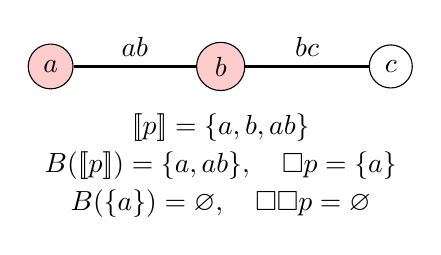
\begin{tikzpicture}[scale=1.2]
  \node[circle,draw,fill=red!20] (a) at (0,0) {$a$};
  \node[circle,draw,fill=red!20] (b) at (1.8,0) {$b$};
  \node[circle,draw] (c) at (3.6,0) {$c$};
  \draw[thick] (a)--node[above] {$ab$}(b)--node[above] {$bc$}(c);
  \node at (1.8,-0.65) {$\llbracket p\rrbracket=\{a,b,ab\}$};
  \node at (1.8,-1.05) {$B(\llbracket p\rrbracket)=\{a,ab\},\quad \Box p=\{a\}$};
  \node at (1.8,-1.45) {$B(\{a\})=\varnothing,\quad \Box\Box p=\varnothing$};
\end{tikzpicture}
\caption{The three-vertex path countermodel witnessing failure of axiom $\mathsf{4}$.}
\label{fig:path-countermodel}
\end{figure}

\begin{rem}
The failure of \(\mathsf{4}\) is structural rather than accidental:
\(\llbracket\Box\varphi\rrbracket_t\) is obtained by composing the
\emph{upward} closure test \(B_t\) on the face poset with the
\emph{downward} operator \(\mathrm{int}_{K_t}\).  Neither factor is
idempotent on the range of the other, so \(\Box\) is not a topological
interior operator and the \(\Box\)-fragment is a normal \(\mathsf{T}\)-logic
strictly weaker than \(\mathsf{S4}\).
\end{rem}

\begin{rem}[Failure of 4 is spatial, not temporal]
\label{rem:box-4-spatial}
The countermodel of Proposition~\ref{prop:box-not-4} uses a single fixed
stage (a constant filtration), so non-transitivity is not an artifact of
the temporal or filtration component.  It arises from composing two
opposite-direction operators on the face poset: \(B_t\) is an upward
test over cofaces, and \(\mathrm{int}_{K_t}\) is a downward
closure-interior operator.  Hence \(\Box\) is not an idempotent
topological interior, and the failure of \(\mathsf{4}\) is a property of
the spatial geometry alone.
\end{rem}

\subsection{Padding constraint}

\begin{rem}[Padding constraint for \(\Box\)]
\label{rem:box-padding}
Since \(B_t(\bot)=\emptyset\) and \(B_t(\top)=K_t\), the two-valued subalgebra
\(\{\emptyset, K_t\}\) is \(\Box\)-closed: \(\Box\emptyset=\emptyset\) and
\(\Box K_t=K_t\).  Hence on extremal (two-valued) valuations,
\(\Box\varphi\leftrightarrow\varphi\) is valid, and padded models cannot
refute \(\Box\)-formulas.  A canonical model for \(\Box\)-completeness must
therefore use \emph{non-extremal} valuations.  This is the main technical
constraint: padding does not break \(\Box\)-validity, it becomes
\emph{insufficient} to refute \(\Box\)-formulas.  We leave
\(\Box\)-completeness w.r.t.\ abstract bi-relational simplicial frames and
a separate \(\Box\)-representation theorem as explicitly open problems.
\end{rem}

\begin{rem}[\(\Box\)-completeness as open problem]
Completeness for the \(L_{\Box}\)-fragment relative to abstract
bi-relational simplicial frames is left as an open problem for
Paper~III.
\end{rem}

%%%%%%%%%%%%%%%%%%%%%%%%%%%%%%%%%%%%%%%%%%%%%%%%%%%%%%%%%%%%%%%%%%%%
\section{Conclusion}
\label{sec:conclusion}

This paper has grounded SC-Logic in a rigorous semantic foundation, closing the gap that Paper~I left open between geometric intuition and formal justification. Four results constitute the core. First, the lattice of subcomplexes of any finite simplicial complex carries a canonical Heyting algebra structure, with the implication given explicitly as the largest subcomplex whose meet with the antecedent is contained in the consequent (Proposition~\ref{prop:heyting-algebra}, Corollary~\ref{cor:heyting-negation}). Second, monotone filtrations induce Kripke frames with persistent valuations, and the simplex-level forcing semantics agrees with the algebraic one over discrete filtrations: truth sets compute exactly the Heyting operations (Proposition~\ref{prop:algebra-kripke-agreement}). Third, the Hilbert-style proof system is sound and complete with respect to the class of filtration models (Theorems~\ref{thm:soundness} and~\ref{thm:completeness}) and enjoys the finite model property (Proposition~\ref{prop:fmp}), from which decidability follows immediately (Corollary~\ref{cor:decidability}). Fourth, moving beyond pure IPC, we isolated the gap between algebraic and Heyting negations (Proposition~\ref{prop:negation-gap}), introduced graded negation along a filtration with its antitone behaviour (Proposition~\ref{prop:graded-antitone}), and defined the clarity operator as the double-negation nucleus, whose fixed points form the Booleanization of the subcomplex algebra (Proposition~\ref{prop:clarity-boolean}).

The relation between this paper and Paper~I is one of foundation to construction. Paper~I established truth-as-geometry operationally: propositions as subcomplexes, inference as topological transformation. The present paper supplies the missing semantics that explain \emph{why} those operations behave intuitionistically. The Heyting algebra of subcomplexes is not a choice of interpretation; it is the canonical structure that the geometry forces. Graded negation makes this precise at the stage level: each filtration step carves out its refutable region, and the erosion of that region as the complex grows is captured algebraically rather than left as geometric intuition.

Taken together, the results identify the propositional, modality-free fragment of SC-Logic exactly with IPC. This identification is not a limitation but a calibration: it tells us precisely what the simplicial-complex geometry is computing when connectives are interpreted topologically, and it marks the boundary at which intuitionistic logic ends and genuinely geometric content begins.

\paragraph{Further directions.}

Several directions remain open for Paper~III. The most pressing is
\(\Box\)-completeness: soundness for the
\(\mathcal{L}_\Box\)-fragment relative to abstract bi-relational simplicial frames
is established, but a representation theorem and full completeness proof remain
open (Section~\ref{sec:box}); this is explicitly positioned as an open problem
rather than a relied-upon result. A second direction concerns robustness
quantification: measuring the persistence interval over which a formula is forced
provides a natural complexity measure for inference, and bottleneck-distance
machinery from persistent homology can be brought to bear on logical consequence
directly. Third, relaxing the monotonicity assumption on filtrations to allow
zigzag filtrations would model revision and retraction of geometric evidence,
requiring a forcing semantics over zigzag persistence modules. Finally, the
computational theory deserves systematic treatment: the complexity of deciding
forcing on finite filtrations, and a computational implementation of this
framework, sketched in Paper~I.

The broader program is a geometric reasoning architecture: logical systems whose
connectives are geometric operations, whose models are evolving spaces, and whose
inferences carry measurable robustness. The results here show that the
propositional, modality-free fragment of spatial reasoning over finite simplicial
complexes is exactly intuitionistic logic, no more, no less, and that everything
beyond it is geometry.
\bibliographystyle{elsarticle-harv}

% Loading bibliography database
\bibliography{references_v2}

\end{document}
